\documentclass[a4paper,11pt]{report}
\usepackage[masterthesis,english]{comp}
\usepackage[english]{babel}
\usepackage{float}
\usepackage{subfigure}

\usepackage{color}
\usepackage{xcolor}
\usepackage{listings}
\usepackage{url}

\usepackage{caption}
\DeclareCaptionFont{white}{\color{white}}
\DeclareCaptionFormat{listing}{\colorbox{gray}{\parbox{\textwidth}{#1#2#3}}}
\captionsetup[lstlisting]{format=listing,labelfont=white,textfont=white}
\lstset{breaklines=true, captionpos=t}

\newcommand{\subscript}[1]{\ensuremath{_{\textrm{#1}}}}
\newtheorem{mydef}{Definition}

% Titel van de master thesis
\title{Domain-Specific Modeling and Model Transformation to support Collaborative Work on Android}

% Jouw naam
\author{Philip De Smedt}

% Promotor / Promotoren
\principaladviser{Prof. dr. Hans Vangheluwe}
\coprincipaladviser{Prof. dr. Juan de Lara}

% Datum waarop de bachelor thesis ingediend wordt
\submitdate{28 mei 2012}

% .bib file (Gebruik JabRef om de file te editeren)
\bibfile{thesis_example}

\begin{document}
\frontpages

\mainbodypages
\chapter{Introduction}

This work has been carried out in cooperation with two academic institutions, University of Antwerp (UA) and Universidad Aut\'onoma de Madrid (UAM).

\section{Problem Description}

The context of this Master's Thesis is Domain-Specific Modeling (DSM) applied to Android development for the generation of collaborative applications. Domain-Specific Modeling and Model Transformation (MT) have the potential to support rapid development and the synthesis of new applications on Android. This thesis investigates the power and limitations of DSM and MT in the context of Android. The metaDepth meta-modeling framework and tool will be used to create a higher level framework that allows the creation of collaborative Android applications.
\\ \\
This work arises from the rising need for mobile applications that solve recurring collaborative problems. We try to tackle those recurring problems by applying DSM on the Android stack to support collaborative work. When a non-technical person previously wanted to solve a problem by means of a smartphone application, this person had to learn how to program. In this framework, we tackled this problem by giving the developer a high-level framework that allows creating a sufficiently complex Android application within hours. The types of applications that can be generated fit specific needs, with a focus on collaboration. Moreover, no knowledge of the Java programming language or the Android SDK are required.

\section{Background}

In general, traditional software development follows a process that aims at guaranteeing a certain standard. Important stages in this process are \textit{specification}, \textit{implementation} and \textit{verification}. Software testing is an important aspect of this latter activity. Although the analysis of different software development processes is out of the scope of this thesis, it is an important contribution to the quality of a solution that solves a problem through DSM. In the following, these three stages are described as a natural evolution to DSM. Also \textit{code generation}, which is used extensively in DSM, will be discussed as a possible solution to recurring software engineering problems.

\subsection{Specification}

Specification identifies the problems a new software system is supposed to solve, its operational capabilities, its desired performance characteristics, and the resource infrastructure needed to support system operation and maintenance \cite{ProcessModels}. Based on the requirements specification, software engineers can build an architectural design. This design can not only be used to build the system, but also has as a goal to create some kind of documentation. If the design truly represents a complete system design, a team of software engineers can proceed to build iterations of the product, dependent on the software lifecycle that is applied \cite{SoftwareDesign}.

\subsection{Implementation}

After creating a requirements specification and any accompanying design documents, a software engineering team can proceed to the implementation stage. An implementation usually is a realization of the design documents created in an earlier step. The result of the implementation stage is a software component or system that conforms as close as possible to those design documents.

\subsection{Verification}

Verification is the process of determining that a system, or a module, meets the specified requirements. Therefore, the verification process always relies on the requirements specification, as this document defines the intended behavior of the system. We should ask ourselves \textit{"Are we building the system right?"}. Verification is usually performed by (automated) testing of the system. The testing process can involve unit testing (testing a component in isolation \cite{UnitTesting}), integration testing (components tested as a group \cite{IntegrationTesting}), regression testing (uncover new errors in existing functionality after changes have been made to a system \cite{RegressionTesting}) and other ways of verifying that the system behaves as we expect it to. Another process closely related to this is \textit{validation}. Validation is the process of determining that a system meets the \textit{actual} requirements of the user. In this process, we should ask ourselves \textit{"Are we building the right system?"}.
\\ \\
A complete software development lifecycle is depicted in figure \ref{fig:lifecycle}. One of the goals of this thesis is to minimize or even eliminate the implementation and testing cycles. Using a DSL, an end-user can easily create and customize their own applications by specifying its functionality in a clear and non-verbose way. This makes the design lifecycle is a lot easier, as the modeling of applications is very rapid and processes several cycles on the background. The activity of generating code is explained in the next subsection.

\begin{figure}[htb]
\centering
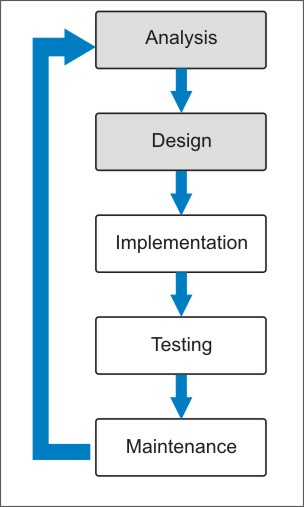
\includegraphics[width=0.6\textwidth]{images/lifecycle.jpg}
\caption{Software Development lifecycle}
\label{fig:lifecycle}
\end{figure}

\subsection{Code Generation}

When developing software, many bugs and errors occur due to coding mistakes in the implementation phase. This can happen due to reusing old software components, unimplemented methods, uninitialized variables, etc. In order to prevent those mistakes, we have to fall back onto coding standards in the development of software systems.
\\ \\
A possible approach is the use of code generation. Among the problems described earlier, it can prevent errors that emerge in manually created code. Usually, a model (e.g. in UML) serves as a blueprint for the generation of the code. Sometimes the code generated from a UML diagram is not complete and merely offers stubs to the users that still have to be implemented manually. The main reason for this is that UML is a generic modeling language. However, if we constrain the required system to a restricted domain, we are able to generate specific code from a DSL. 

\section{Contribution}

\subsection{Aims and Objectives}

The goal of this Master's Thesis is to provide a coherent modeling framework for the creation of collaborative applications running on the Android platform. 
\\ \\
These are the main objectives of the study:

\begin{itemize}
\item{Discuss the shortcomings of two level modeling and why we need multi-level modeling}
\item{Analyze the possibilities of model driven engineering in the context of the Android platform}
\item{Analyze and define the different types of collaboration methods}
\item{Create a coherent framework that allows the creation of collaborative Android applications}
\end{itemize}

\subsection{Research Questions}

The research questions are sustained on underlying hypotheses. The following are the main hypotheses with accompanying research questions:

\begin{itemize}
\item{Hypothesis 1. Android is an open source software stack. \\
Research Question 1. How can we leverage the Android stack to support the modeling of Android applications?}
\item{Hypothesis 2. There exists a categorization of different types of groupware. \\
Research Question 2. How can we support the different types of groupware in a modeling framework?}
\item{Hypothesis 3. We have a broad offering of collaborative applications and functionalities are offered as separate applications. \\
Research Question 3. How can we integrate different functionalities in one collaborative application that is adaptable to a group of people?}
\end{itemize}

\subsection{Expected Outcomes}

These are the expected outcomes for this thesis:

\begin{itemize}
\item{A study of the possibilities of multi-level meta-modeling}
\item{A study of the possibilities of modeling Android applications}
\item{An ontology of collaboration patterns (the collaboration stack)}
\item{A standardization of collaborative patterns in a framework}
\item{A description and design of a modeling framework for collaborative applications}
\end{itemize}

\section{Thesis Outline}

This document starts with an overview of the fundamentals of domain specific modeling in chapter 2. It also explains why there are shortcomings in the two-level modeling approach. Chapter 3 continues with a solution (multi-level modeling) that resolves problems inherent to two-level modeling. We illustrate these problems using the Metadepth multi-level modeling framework. In chapter 4, the main components of Android are discussed, such as Activities and the AndroidManifest file that is a blueprint for Android components in an application. Chapter 5 discusses the different collaborative methods such as Groupware, Computer-Supported Cooperative Work (CSCW) and Computer-Supported Collaborative Learning (CSCL). Using the concepts we have learned from chapter 5, we can make a complete framework with the appropriate collaborative patterns included in chapter 6. This chapter will contain all the designs that make the entire collaborative modeling framework. Chapter 7 proposes a case study where we have developed a complete application using the collaborative modeling framework. The application allows a group of users to authenticate (and thus initiate a session) and collaborate with each other on a certain research project. They can communicate asynchronously (by adding list items or comments on research papers) as well as synchronously (chatting). Finally, chapter 8 concludes the thesis and talks about future work.

\chapter{Domain Specific Modeling}

Domain-Specific Modeling is a software engineering methodology for designing and developing complex systems. Modeling a system through a domain-specific language (DSL) allows the user to rapidly iterate through different prototypes and represent them at various levels of abstraction. The goal of this chapter is to give the reader an introduction to DSM and the primary meta-modeling technology, the Unified Modeling Language (UML) framework. 
\\ \\
Modern software design has reached a complexity that requires well-defined engineering methods and model-based approaches to ensure correctness. Complex systems are becoming extremely heterogeneous and the many engineering disciplines that are involved in system design all require problem-specific formalisms. As such, a company may resort to modeling techniques to solve complex problems in a specific way.
\\ \\
The most common way for creating domain models is through the modeling language standard, UML. Creating a domain model in UML essentially consists of composing a model through one or more class diagrams, capturing the important domain concepts and their relationships. The main objective of this chapter is to address issues with the object-oriented paradigm currently underpinning the UML. UML supports modeling at two levels only, e.g. in the form of class diagrams (type level) and object diagrams (instance level). Thus, it provides only meager support for true multi-level modeling. As a consequence, this two-level modeling approach adds accidental complexity to domain models \cite{AccidentalComplexity}. Solutions for this problem will be discussed in chapter 3, Deep Meta-Modeling.
\\ \\
In the next section, traditional approaches to meta-modeling will be discussed. We continue with the shortcomings and problems of the UML Modeling Framework and current meta-modeling techniques. An example domain model will be presented and used throughout consecutive sections. This example will be based around a computer hardware product hierarchy and can be described in several ways.
\\ \\
Furthermore, the main issues introduced by the \textit{strict} meta-modeling approach, inherent to the UML Framework, will be discussed. These issues arise from the need to capture both \textit{classlike} and \textit{objectlike} features of model elements in two modeling levels. As a consequence, the modeler introduces a mismatch between the problem and the technology used to represent this problem. A mismatch that makes models more complex than they need to be, and by which \textit{accidental complexity} is introduced. Solutions for avoiding this accidental complexity will be discussed in depth in chapter 3.

\section{Traditional Meta-Modeling}

This section discusses traditional meta-modeling approaches that are used in domain specific modeling. Before we dive into the UML modeling framework, we need to define what a formalism is and how meta-modeling is used to describe a formalism.

\subsection{Formalism}

A formalism typically consists of a \textit{syntactic} part and a \textit{semantic} part. The syntax of the formalism deals with form and structure. Additionally, the syntactic part is separated into a \textit{concrete} and \textit{abstract} part. The concrete syntax relates to the actual appearance of the language elements (graphical or textual). The abstract syntax pertains to how the language components may be connected. For example, a Petri Net Transition may only be connected to a Petri Net Place. \\ \\
The semantic part on its turn relates to the \textit{meaning} of the syntactic constructs. The semantic part is also separated in two parts, \textit{operational} and \textit{denotational}. The operational part explicitly captures how a model can be executed. With a denotational specification, we can provide rules to map a model in a given formalism onto a model in a different formalism for which a semantics is available. We can for example map a Statechart to its equivalent Petri Net. Both semantic approaches ultimately define a transformation.

\subsection{Meta-Modeling}

Meta-modeling concentrates on the modeling of modeling formalisms. To solve domain specific problems as fast as possible, explicitly modeling the formalisms is the most efficient approach. Additionally, meta-modeling exhibits lots of other advantages. First of all, a modeling environment may be generated from a meta-model by a set of language tools. A model of a modeling language can also serve as documentation and as a specification. Additionally, by modifying a meta-model, new domain-specific languages can be designed in an easy manner. Last but not least, the generation of a modeling tool through a meta-model is possibly orders of magnitude faster than developing such a tool by hand. This generated modeling tool will most likely be less error prone too \cite{CAMPaM}. \\ \\
Meta-models are models on their own, so they must be specified in a modeling language. This modeling language is specified by a meta-meta-model. Most of the time, UML class diagrams are used to express the meta-model. On their own, UML class diagrams are expressive enough to be expressed by themselves, e.g. UML is partly defined in terms of UML. This so-called \textit{meta-circularity} refers to the fact that the meta-model of a language L is a model in language L.

\subsection{Linear Modeling Hierarchy}

In this section, we briefly discuss the UML Modeling Framework. First, we present the four-layered Meta-Object Facility (MOF) along with a small example. \\ \\
The overall architecture of the UML modeling framework is most heavily influenced by the CASE Data Interchange Format (CDIF) standard developed by a consortium of CASE tool vendors\footnote{CASE Tools: Computer-Aided Software Engineering Tools}. The CDIF standard describes the different modeling languages used to create specific user models in terms of a single fixed, core model (a meta-meta-model) \cite{RearchitectingUML}. The meta-modeling architecture is depicted in figure ~\ref{fig:mm_architecture}.
\begin{figure}[h!]
\centering
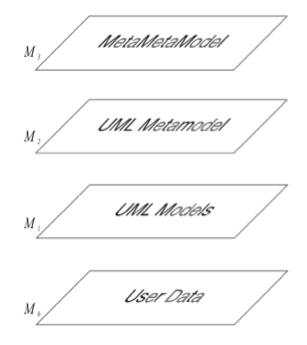
\includegraphics[width=0.4\textwidth]{images/mm_architecture.png}
\caption{The four-level meta-modeling architecture}
\label{fig:mm_architecture}
\end{figure}
The meta-meta-model (M\subscript{3}) level is the highest level, from which the UML meta-model is created. In general, it is the core from which the descriptions of specific modeling languages (i.e. specific language meta-models) are created. The UML meta-model (M\subscript{2}) describes the core from which specific language meta-models are created. Specific models are then created as instances of these language meta-models on the M1 level. The User Data depicts instances of such models created in M\subscript{1}. An example of this approach can be seen in figure ~\ref{fig:two_level_inst}.
\begin{figure}[h!]
\centering
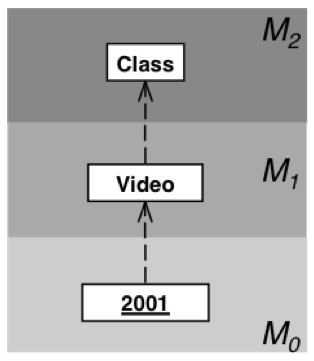
\includegraphics[width=0.4\textwidth]{images/chap2_two_level_inst.png}
\caption{Extending the two levels of instantiation}
\label{fig:two_level_inst}
\end{figure}
In this example, the dashed arrows in the figure describe an "instance of" relationship. Every level in the diagram is an instance of its level above. For example, an instantiation of the concept Video resides at level M\subscript{0}. Video on its turn is an instantiation of Class and Class is regarded as an instance of the meta-meta-model elements (the M\subscript{3} level, not shown in this example).

\subsection{Linguistic Meta-Modeling}

In the meta-modeling field, we can distinguish two different approaches of meta-modeling, linguistic and ontological meta-modeling. The linguistic approach relegates ontological instance-of relationships, which relate user concepts to their domain types, to a secondary role \cite{MDDFound}. A linguistic instance-of relationship crosses a linguistic metalevel, whereas ontological instance-of relationships do not cross such levels. Ontological instance-of relationships merely relate entities within a given level. Figure ~\ref{fig:ling_mm} shows this interpretation of the four layered architecture as embraced by the UML and MOF standards. 
\begin{figure}[h!]
\centering
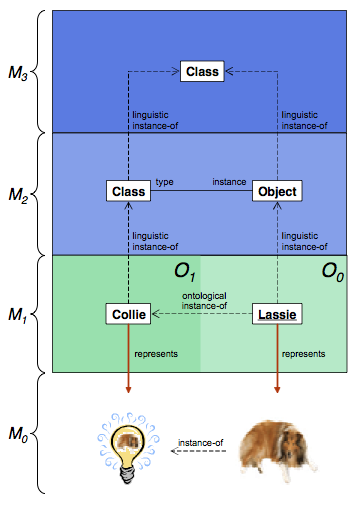
\includegraphics[width=0.6\textwidth]{images/chap2_linguistic_mm.png}
\caption{Linguistic meta-modeling \cite{MDDFound}}
\label{fig:ling_mm}
\end{figure}

\subsection{Ontological Meta-Modeling}

When we want to dynamically extend a modeling language, only linguistic meta-modeling doesn't suffice. Modeling language extensions are facilitated as dynamic user extensions, introducing the need for ontological meta-modeling. This dynamic requirement in turn requires the capability to define domain metatypes (i.e. types of types). We refer to this form of meta-modeling as ontological meta-modeling since it is concerned with describing what concepts exist in a certain domain and what properties they have \cite{MDDFound}. \\ \\
When we take a look back at figure ~\ref{fig:ling_mm}, we already see an ontological instantiation example. The model element \texttt{Lassie} is an ontological instance-of relationship of \texttt{Collie}, and thus resides at a lower ontological level than \texttt{Collie}. This expresses the fact that in the real world, the mental concept \texttt{Collie} is the logical type of \texttt{Lassie} \cite{MDDFound}. Figure ~\ref{fig:ling_mm} only contains two ontological levels, both contained within the linguistic level M\subscript{1}. We can extend the ontological approach among multiple levels too. This is featured in figure ~\ref{fig:ont_mm}, where we introduce three ontological levels. In ontological level O\subscript{2}, we show that \texttt{Collie} can be regarded as an ontological instance of \texttt{Breed}. The ontological metatype \texttt{Breed} not only distinguishes types like \texttt{Collie} and \texttt{Poodle}, but also from other types (such as \texttt{CD} and \texttt{DVD}). Moreover, we can also use this metatype to define breed properties, for example, where a particular breed first originated.
\begin{figure}[h!]
\centering
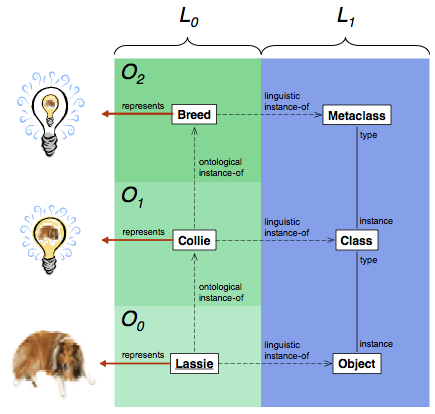
\includegraphics[width=0.6\textwidth]{images/chap2_ontological_mm.png}
\caption{Ontological meta-modeling \cite{MDDFound}}
\label{fig:ont_mm}
\end{figure}
\newpage

\section{Strict Meta-Modeling}

In the following section, we will discuss strict meta-modeling and the fundamental problems it exhibits are introduced.

\subsection{Definition}

The linear modeling approach described in the previous section exhibits a number of fundamental problems. One of them is the fact that the precise meaning of the instance-of relationship is not defined. The UML documentation does not contain a formal definition of the instance-of relationship. It merely states that a modeling level in the hierarchy must be an instance of its level above. Therefore, a formal concept should be defined to encapsulate the exact meaning of the instance-of relationship. This concept is formalized through strict meta-modeling. Strict meta-modeling states that if a model A is an instance-of another model B, then every element of A must be an instance-of some element in B \cite{RearchitectingUML}. This concept is illustrated in figure ~\ref{fig:strict_mm}. Here we see that strict meta-modeling interprets the instance-of relationship at the level of individual model elements. As a consequence, modeling levels have strict boundaries and may be crossed only by instance-of relationships.
\begin{figure}[h!]
\centering
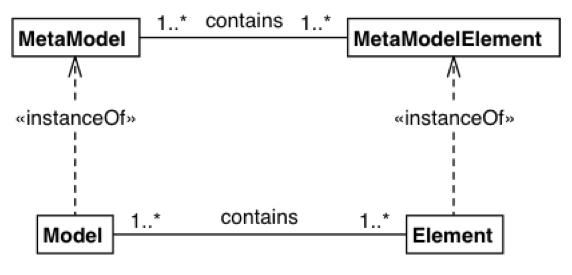
\includegraphics[width=0.7\textwidth]{images/chap2_strict_mm.png}
\caption{Strict meta-modeling.}
\label{fig:strict_mm}
\end{figure}
The exact definition of strict meta-modeling is defined as follows:
\begin{mydef}
In an \textit{n}-level modeling architecture, M\subscript{0}, M\subscript{1}, ..., M\subscript{n-1}, every element of an M\subscript{m}-level model must be an instance-of exactly one element of an M\subscript{m+1}-level model, for all \textit{0} $\leq$ \textit{m} $\le$ \textit{n-1}, and any relationship other than the instance-of relationship between two elements \textit{X} and \textit{Y} implies that level(X) = level(Y).
\end{mydef}
It is clear that the topmost level \textit{n} is ignored in this definition. Nevertheless, we can model the top level so that its elements are instances of themselves, such that we can terminate the hierarchy of meta-levels.

\subsection{Limitations of Strict Meta-Modeling}

There are several issues with the existing UML modeling framework, such as \textit{dual classification} and the \textit{class/object duality} \cite{RearchitectingUML}. The class/duality problem arises from the need to capture both classlike and objectlike facets of some model elements in one level and dual classification is based on the fact that we need to capture both logical (e.g. \texttt{Video}) as well as physical (e.g. \texttt{Object}) aspects of model elements. Every solution to these problems ultimately leads to unwanted, accidental complexity. Those solutions try to include multiple programming levels into a single modeling level, due to the limitations of strict meta-modeling. In what follows, we will focus on both the class/duality problem and the dual classification problem. For example, one could note that in figure ~\ref{fig:two_level_inst}, the M\subscript{2} level aims to address two concerns. This problem is denoted in figure ~\ref{fig:multiple_class_mm}. Here, user types at the M\subscript{0} level are defined as instances of two concepts. First, the \textit{2001} instance is an instance of the M\subscript{1}-level type \textit{Video}, and second of the M\subscript{2}-level meta-type Object. Although this approach feels natural, it is clearly in violation with our definition of strict meta-modeling:

\begin{itemize}
\item{Object 2001 has more than one classifier (Video and Object).}
\item{An instance-of relationship crosses more than one meta-level boundary.}
\end{itemize}

\begin{figure}[h!]
\centering
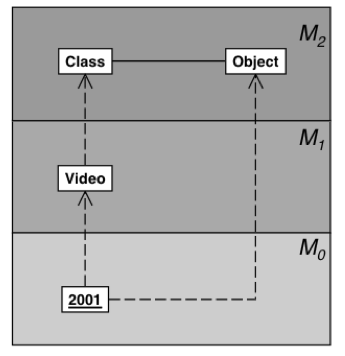
\includegraphics[width=0.4\textwidth]{images/chap2_multiple_class_uml.png}
\caption{Multiple classification in the current UML framework.}
\label{fig:multiple_class_mm}
\end{figure}

It is clear that we have to modify our approach to strict meta-modeling. The following section addresses the issues in which accidental complexity occurs and provides well-defined solutions for them.

\section{Problems with the two-level UML Modeling approach}

In this section, we will introduce an example domain model. We will also demonstrate a few workarounds used to represent multi-level domain models using only two modeling levels.

\subsection{Example domain model}

This sample model adopts a computer hardware product hierarchy using the "Item Description" pattern. This example exhibits a typical technique which is often used to capture a multi-level domain classification into the two-level UML modeling style. The example class diagram is depicted in figure ~\ref{fig:cd_itemdesc}.
\begin{figure}[h!]
\centering
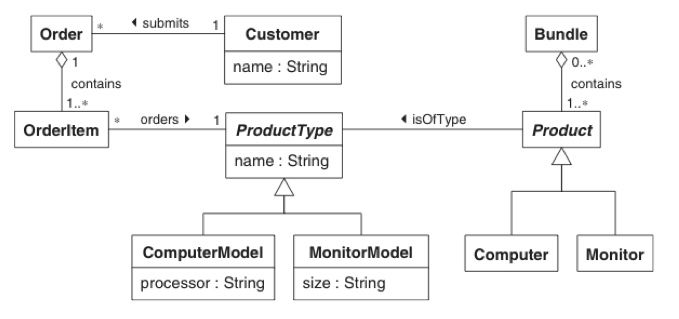
\includegraphics[width=0.9\textwidth]{images/chap2_cd_itemdesc.png}
\caption{Example class diagram of the Item Description pattern.}
\label{fig:cd_itemdesc}
\end{figure} \\
The above class diagram is separated into two parts. One part models products sold by an enterprise and the other part models the descriptions of these products. Here, instances of \texttt{ProductType} (\texttt{ComputerModel} and \texttt{MonitorModel}) are descriptions of the \texttt{Product} types (Computer and Monitor). The idea is to let objects play the role of classes in order to explicitly represent class-level information \cite{AccidentalComplexity}. In this way, we can dynamically change information about a product and keep this information even when no representation of this product type exists. An example of an instance of the above class diagram is depicted in figure ~\ref{fig:domain_instance}.
\begin{figure}[h!]
\centering
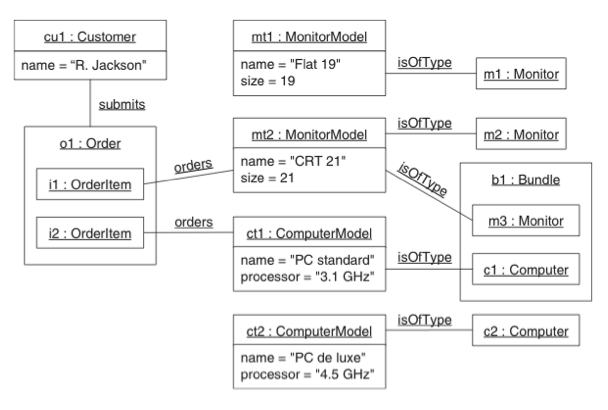
\includegraphics[width=0.9\textwidth]{images/chap2_domain_instance.png}
\caption{Domain instance (object diagram).}
\label{fig:domain_instance}
\end{figure} \\
The \texttt{isOfType} links between \texttt{Monitor} / \texttt{Computer} instances and \texttt{MonitorModel} / \texttt{ComputerModel} instances conceptually represent a form of \textit{instance-of} relationship (as explained in previous section), although all objects involved in the example are at the instance level in an object diagram. This verbosity does not violate strict meta-modeling, but introduces a workaround at the object level in order to create new objects at runtime.

\subsection{Domain types as objects}

We have used the graphical \texttt{isOfType} links to model the instance/type relationships at the object level. However, we can distinguish up to three different kinds of instance-of relationships:

\begin{itemize}
\item{the UML built-in \textit{instance-of} relationship between the elements in the object diagram and the elements in the class diagram (e.g. \texttt{m1} \textit{instance-of} \texttt{Monitor})}
\item{the \texttt{isOfType} associations in the class diagram between \texttt{Product} classes and \texttt{ProductType} classes (e.g. \texttt{Computer} \textit{isOfType} \texttt{ComputerModel})}
\item{the \texttt{isOfType} links between instances of \texttt{Product} and instances of \texttt{ProductType} (e.g. \texttt{c2} \textit{isOfType} \texttt{ComputerModel})}
\end{itemize}
Undoubtedly, the combination of these relationships introduce some kind of accidental complexity. To see the consequences caused by this approach, we have combined the object and class diagram in one figure that explicitly represents all the relationships that conceptually exist. This diagram can be found in figure ~\ref{fig:class_object_diagram}. This figure actually highlights two aspects of the two-level modeling paradigm that was not explicitly clear from the separate diagrams:

\begin{itemize}
\item{It shows all UML \textit{instance-of} relationships explicitly in addition to the \texttt{isOfType} relationships.}
\item{It highlights the fact that the object diagram contains model information that represents domain instances and types of the domain conceptualization.}
\end{itemize}
The black dots in the figure below the dashed lines represent the domain entities. On the one hand, we have got domain types and on the other hand, we have got domain instances. The relationships between the domain entities use the same \textit{instance-of} relationships as between the model types and model instances. They represent \textit{ontological} \textit{instance-of} relationships, because they show which domain entities are considered to be types of other domain entities.
\begin{figure}[h!]
\centering
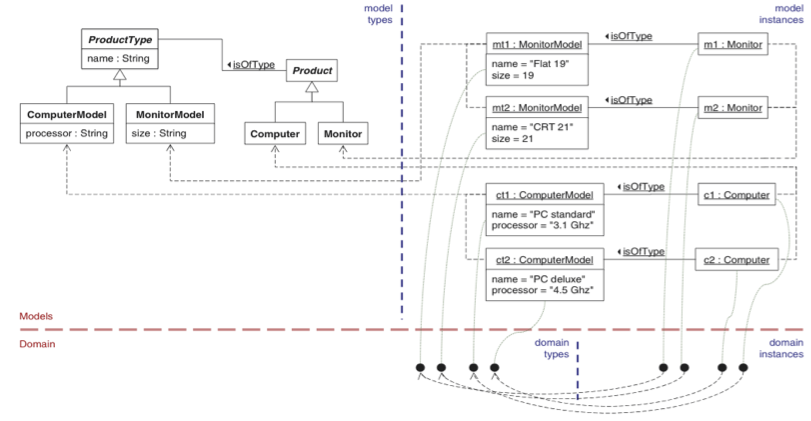
\includegraphics[width=1.0\textwidth]{images/chap2_class_object_diagram.png}
\caption{Combination of the class and object diagram.}
\label{fig:class_object_diagram}
\end{figure} \\
After investigation of the figure above, we see that it contains some redundant information. There are some model elements that do not represent any domain elements. Type \texttt{Product} and its subclasses can be considered as abundant model attributes if the model is interpreted as a domain model, because they have two classification relationships instead of just one. The subclasses \texttt{Computer} and \texttt{Monitor} merely exist to set up the \textit{Item Description} pattern. For instance, \texttt{m1} has type \texttt{Monitor} plus a modeled type \texttt{mt1}. The redundancy introduced here is an example of accidental complexity, because some information only exists to realize some workaround technique.

\subsection{Domain types as classes}

The model presented in the previous subsection is often used when we need to introduce new types of products dynamically. When we do not need to create objects dynamically at runtime, we can simplify the model significantly. This approach is shown in figure ~\ref{fig:types_classes}. It shifts some modeling elements that represent domain types (i.e. \texttt{mt1}) to the type level (into the class diagram). According to the UML class/object modeling conventions, this is a more natural place for these elements to be.
\begin{figure}[h!]
\centering
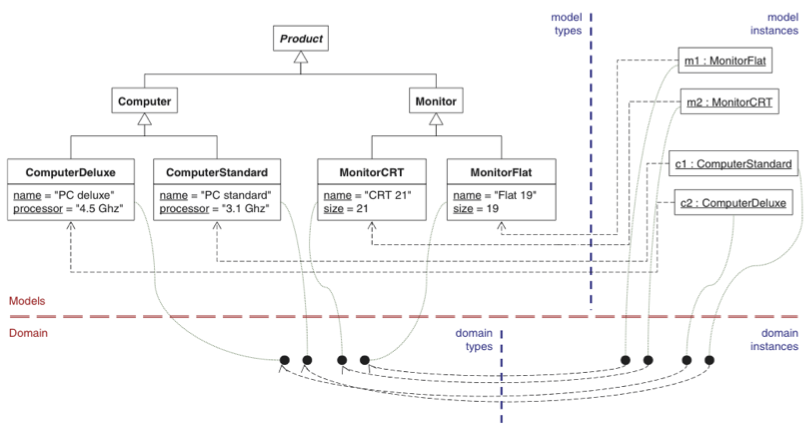
\includegraphics[width=1.0\textwidth]{images/chap2_types_classes.png}
\caption{Types as classes.}
\label{fig:types_classes}
\end{figure} \\
Although the figure above removes some accidental complexity from the previous example, we also lost some features. It is no longer possible to instantiate new types at runtime, because product types are now represented by classes. Without additional information, we cannot conclude whether the workaround methods of previous section were necessary or not. Therefore, it is hard to compare the models and evaluate them on the level of accidental complexity. In the next chapter we will see whether it is possible to keep the simplicity of figure ~\ref{fig:types_classes} and still support the ability to create new product types at runtime.

\chapter{Multi-Level Modeling and Metadepth}

This chapter continues where chapter 2 left off. Now that we know we can capture the important domain concepts and their relationships through the modeling language standard UML, we can address issues with the object-oriented paradigm currently underpinning the UML. UML supports modeling at two levels only, e.g. in the form of object diagrams (instance level) and class diagrams (type level). Thus, it provides only meager support for true multi-level modeling. As a consequence, this two-level modeling approach adds accidental complexity to domain models. A possible solution involves the use of powertypes. Another solution is to introduce an object that can both capture \textit{classlike} and \textit{objectlike} features, \textit{clabjects}, together with the concept of potency to support an arbitrary number of modeling levels. Both concepts are explained in depth. Finally, Metadepth, a framework for multi-level meta-modeling is presented. This approach is trying to solve the mismatch between the �two level� modeling paradigm and the information it models.

\section{Deep Meta-Modeling}

A question that undoubtedly comes to ones mind is the following: "Is it possible to keep the simplicity of figure ~\ref{fig:types_classes} and still support the ability to create new product types at runtime?". In order to make this possible, the type level should be as dynamic as the object level. We should of course have some control over what types are created and what features they possess. Therefore, we need (domain-)meta-types controlling the features of (domain-) types \cite{AccidentalComplexity}. However, the problem with the "Item Description" pattern is that it uses three classification levels, where only two level (class/object) mechanisms are supported. This introduces a level mismatch problem, depicted in figure ~\ref{fig:mapping_inconsistent}. It shows that our example actually features \textit{three} ontological levels, while the corresponding models only contain \textit{two} modeling levels. The level of the model instance is used to represent two ontological levels, domain types and domain instances.

\begin{figure}[h!]
\centering
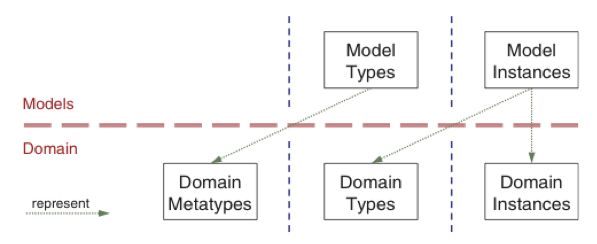
\includegraphics[width=0.9\textwidth]{images/chap3_mapping_inconsistent.png}
\caption{Mapping domain levels to modeling levels.}
\label{fig:mapping_inconsistent}
\end{figure}

In the following, we will discuss how it is possible to avoid squeezing multiple domain levels in only two modeling levels.

\subsection{Clabject}

In order to truly support multiple levels, modeling concepts that can be applied in a uniform way across all levels in a multilevel hierarchy should exist \cite{AccidentalComplexity}. A modeling construct that supports the representation of the dual �type and object�-property of some domain concept is necessary. Therefore, the concept of \textit{clabject} was introduced. Clabjects are a combination of \textit{class} and \textit{object}. They have a name and a set of attributes, like classes, and a set of slots, like objects. The example of previous section, modeled using clabjects, is depicted in figure ~\ref{fig:model_clabject}. This solution features less accidental complexity than solutions of previous sections, because it maximizes the mapping between the problem structure and the solution structure. Note that the model types do not contain attributes, they only fill in slots, and subsequently instances do not contain any slots. Furthermore, we have used only a single notion of the \textit{instance-of} relationship.

\begin{figure}[h!]
\centering
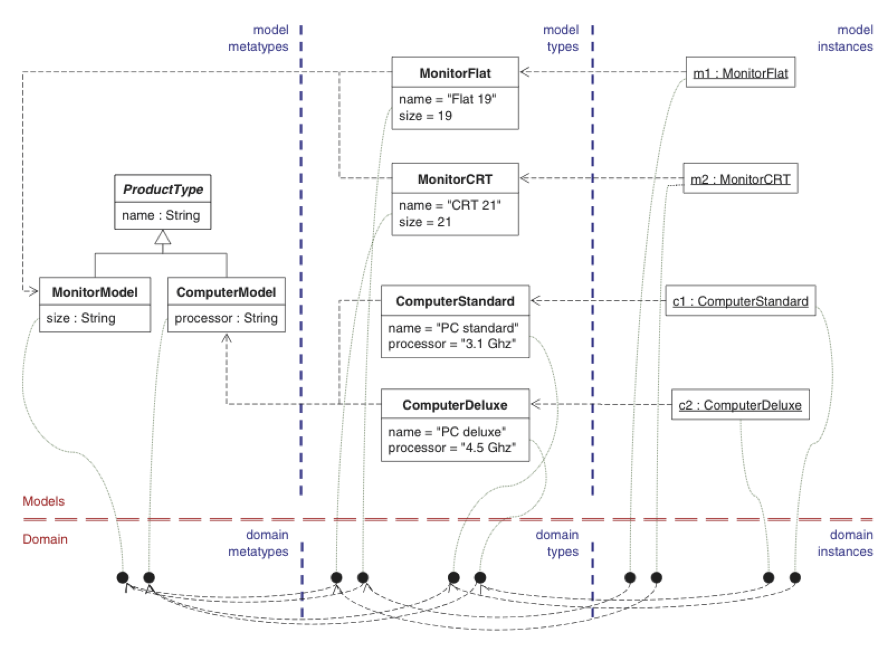
\includegraphics[width=0.9\textwidth]{images/chap3_model_clabject.png}
\caption{Example modeled using clabjects.}
\label{fig:model_clabject}
\end{figure}

Clabjects support any number of model classification levels, which creates a \textit{direct mapping} between ontological domain levels and modeling levels. This concept is visualized in figure ~\ref{fig:mapping_clabject}. This direct mapping requires that the solution structure reflects the problem structure as close as possible. Now that we have introduced clabjects, a uniform way to support multiple domain levels, we can address the issue when elements in one level need to influence elements beyond its neighboring levels.

\begin{figure}[h!]
\centering
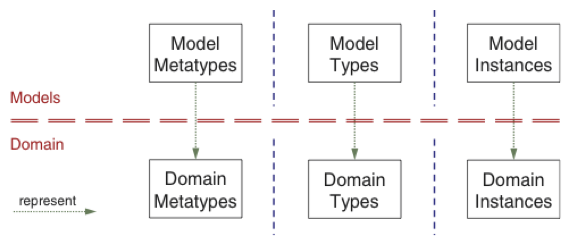
\includegraphics[width=0.9\textwidth]{images/chap3_mapping_direct.png}
\caption{Direct mapping between ontological domain levels and modeling levels.}
\label{fig:mapping_clabject}
\end{figure}

\subsection{Powertypes}

Using clabjects, the accidental complexity in the domain model was reduced significantly. However, there is one additional issue that needs to be addressed to allow multiple classification levels to be modeled naturally. This is the issue of \textit{deep characterization}. Deep characterization means that a type can influence the attributes of its instances� types as well as their object facets. Figure ~\ref{fig:deep_powertypes} shows an example of how powertypes can be used to represent deep characterization. If a superclass (e.g. \texttt{Computer}) is said to have a powertype (\texttt{ComputerModel}), then an instance of the powertype (\texttt{ComputerStandard}) is only well-formed when it inherits from the superclass (\texttt{Computer}). Every derived class of a class inheriting from a powertype should also be an instance of that powertype (e.g. \texttt{ComputerDeluxe} inherits from \texttt{Computer} and is also an instance of the powertype \texttt{ComputerModel}). Hence, all subclasses in our example will have a \texttt{processor} or \texttt{size} \textit{slot} and a \texttt{price} or \texttt{picQlty} \textit{attribute}. For example, the \texttt{size} attribute of \texttt{MonitorModel} is a slot in \texttt{MonitorFlat}, because it is an instance of \texttt{MonitorModel}. Powertypes therefore control the type facet of powertype instances by means of inheritance. The powertype mechanism supports deep characterization, but as can be seen in the example only at the cost of introducing supertypes whose only purpose might be to provide a type facet for their subclasses. In the next section, we will solve this accidental complexity by introducing \textit{deep instantiation}.

\begin{figure}[h!]
\centering
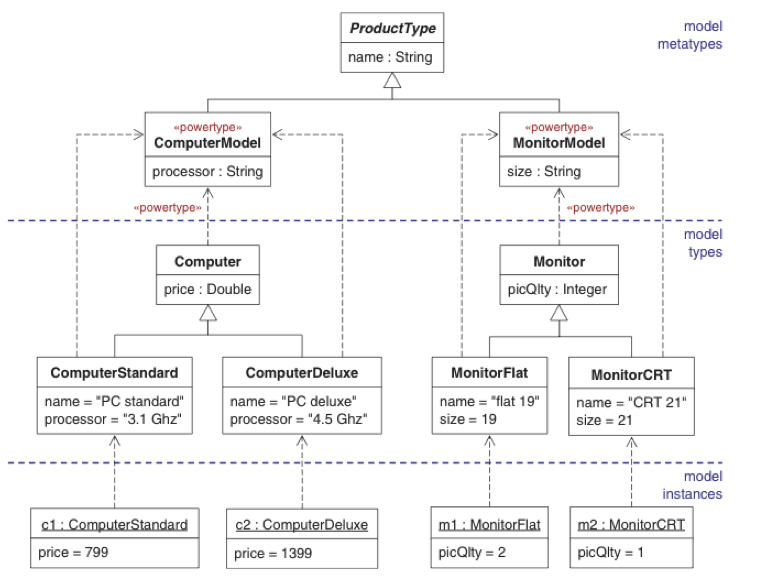
\includegraphics[width=0.9\textwidth]{images/chap3_deep_powertypes.png}
\caption{Deep characterization with powertypes.}
\label{fig:deep_powertypes}
\end{figure}

\subsection{Deep Instantiation}

Deep characterization exists when a type should influence an entity beyond its immediate instances. In order to support deep characterization, we need a mechanism that backs it up in a concise way and minimizes accidental complexity introduced by deep characterization with powertypes. This mechanism is referred to as \textit{deep instantiation}.

\subsubsection{Potency}

Deep instantiation covers two concepts. One is the unification of attributes and slots into a single concept, which we refer to as \texttt{field}. The other concept extends clabjects and fields with an additional property known as \textit{potency}. Potency defines how deep an instantiation chain produced by a clabject or field may become. For example, when we create a field of potency two, it can produce an instantiation depth of two. Each instantiation of the field lowers the potency value by one, until the potency value equals zero. Entities with potency zero cannot be further instantiated and act like regular objects or slots. Figure ~\ref{fig:deep_potency} shows our domain model represented by deep characterization.

\begin{figure}[h!]
\centering
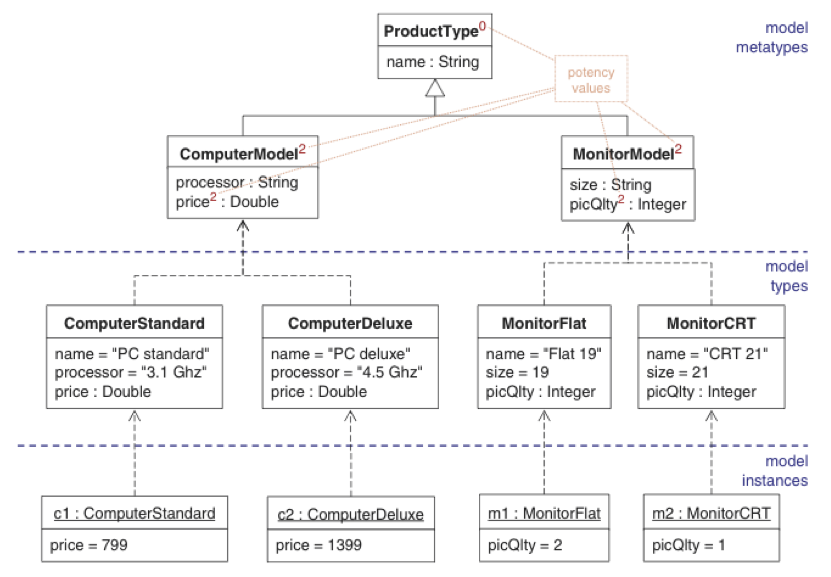
\includegraphics[width=0.9\textwidth]{images/chap3_deep_potency.png}
\caption{Deep characterization with potency.}
\label{fig:deep_potency}
\end{figure}

The clabject \texttt{ComputerModel} has a field \texttt{price} of potency two at the model metatypes level. This is indicated by the superscript \textit{2} at the field \texttt{name}. After instantiating the clabject once, the potency of field \texttt{price} is reduced by one. Note that �price� acts like an attribute on this level (indicated by a potency of 1). When we instantiate this clabject to an object \texttt{c1}, field \texttt{price} has turned into a slot that has a real value. Note that a potency value of zero for clabjects with non-zero potency fields allow us to create an \textit{abstract} (meta-)class.
\\ \\
The example using potency features the least accidental complexity yet. It only allows computer and monitor types for computer and monitor instances respectively, without enhancing it with extra constraints. Furthermore, it doesn�t require an extra superclass for merely providing a type facet like with powertypes.

\section{Metadepth}

MetaDepth is a meta-modeling framework written in Java that uses a deep meta-modeling approach to support multiple programming levels. It allows a developer to work in two ontological (domain) instantiation modes: \textit{strict} and \textit{extensible}, as shown in figure ~\ref{fig:metadepth_schemes}.

\begin{figure}[h!]
\centering
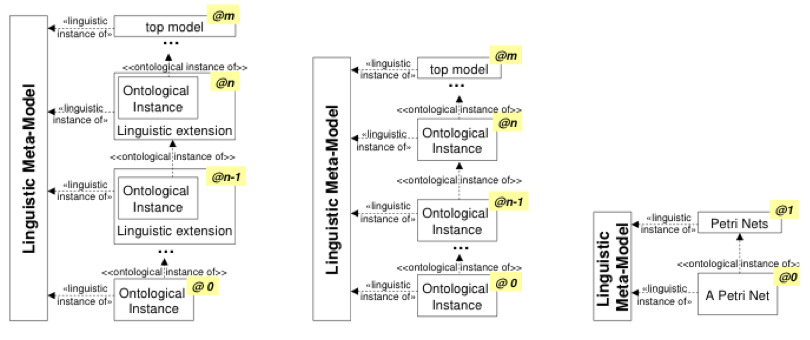
\includegraphics[width=0.9\textwidth]{images/chap3_metadepth_schemes.png}
\caption{MetaDepth instantiation schemes: extensible ontological instantiation (left) and strict ontological instantiation (center). Example of strict instantiation (right).}
\label{fig:metadepth_schemes}
\end{figure}

In the extensible case, it is possible to linguistically extend each ontological instance model (as depicted in the figure). This means that instances of elements marked as \texttt{ext} can be extended with new attributes. We can also mark a complete model as extensible, allowing us to add new types and extend its elements. The alternative \textit{strict} case is similar to most meta-modeling environments in the sense that the top-level meta-model hardcodes all language concepts and can be subsequently instantiated. This is depicted in the center of figure ~\ref{fig:metadepth_schemes}.

\subsection{The Linguistic Meta-Model}

MetaDepth uses its own linguistic meta-model, inspired by MOF \cite{MetaDepth}. It�s modified to accommodate an arbitrary number of meta-levels, deep instantiation and potency. Part of the linguistic meta-model is shown in figure ~\ref{fig:metadepth_schemes}. The uncolored classes are those the designer usually instantiates when building his own model.

\begin{figure}[h!]
\centering
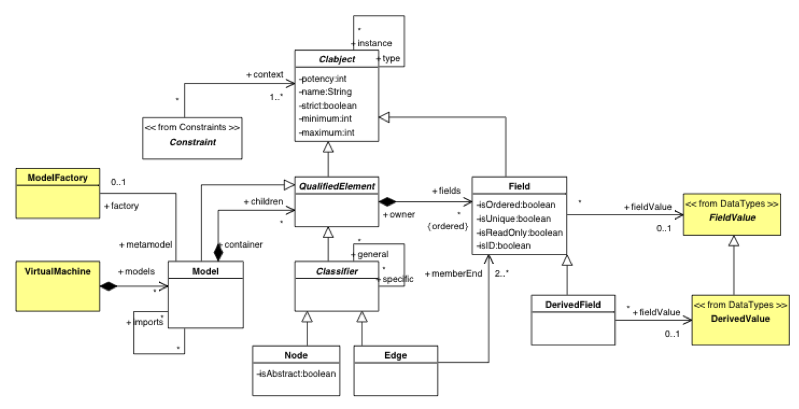
\includegraphics[width=0.9\textwidth]{images/chap3_metadepth_mm.png}
\caption{MetaDepth�s linguistic meta-model.}
\label{fig:metadepth_schemes}
\end{figure}

The root class \texttt{Clabject} takes responsibility of handling the dual type/object facet of elements \cite{MetaDepth}. Therefore, it contains a potency attribute and links to its instances and types. \texttt{Constraints} can be attached to clabjects, as shown in the class diagram. All working models are managed by a \texttt{VirtualMachine} container, which is a \textit{singleton} object. An example of the dual classification using a clabject and the two instance-of relationships is shown in figure ~\ref{fig:dual_class}. The ontological model stack depicts the user-defined (meta-)models, instantiated through the linguistic meta-model shown above.

\begin{figure}[h!]
\centering
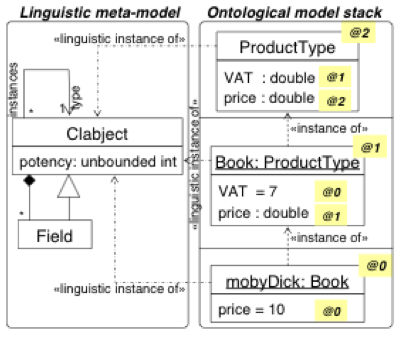
\includegraphics[width=0.4\textwidth]{images/chap3_dual_class.png}
\caption{Dual classification example.}
\label{fig:dual_class}
\end{figure}

\subsection{Tool Support}

MetaDepth models can be built through a Java API or through a \texttt{CommandShell} and a textual syntax, built with ANTLR \cite{ANTLR}. The storage of models is also done in this format. As an example, figure ~\ref{fig:model_ex} shows the three model dual classification example of figure ~\ref{fig:dual_class} in the textual notation. In this example, the model Store (with potency two) is extended linguistically through the Node \texttt{ProductType}. The VAT attribute in node \texttt{ProductType} has a potency of one (and a default value of 7.5), which means that it will be instantiated in its lower neighboring level. We could also declare \textit{anonymous} clabjects, like \texttt{Book\{price=10;\}}.

\begin{figure}[h!]
\centering
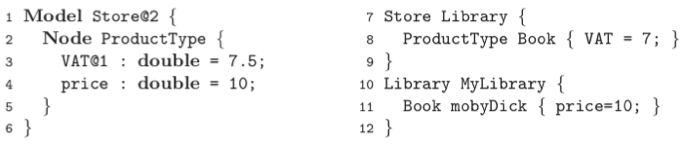
\includegraphics[width=0.9\textwidth]{images/chap3_model_ex.png}
\caption{Three model example.}
\label{fig:model_ex}
\end{figure}

The Metadepth framework is integrated with Epsilon, a family of languages built on top of the Epsilon Object Language (EOL) \cite{EclipseEOL}, by communicating with the models through a connectivity layer. EOL can work with EMF models \cite{EclipseEMF}, but also with any other model technology that implements the interface of this connectivity layer. Metadepth works through this kind of interface and adds support to make EOL aware of multiple ontological levels. Using this approach, we can use EOL programs to create models, as shown in figure ~\ref{fig:eol}. We could also use EOL to define the semantics of a model (e.g. write a Petri Net simulator based on a model using the Epsilon Transformation Language (ETL) \cite{EclipseETL}).

\begin{figure}[h!]
\centering
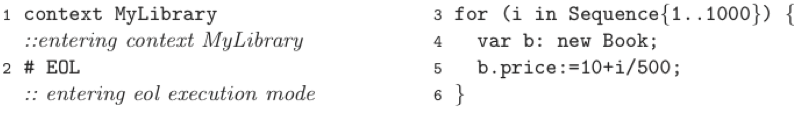
\includegraphics[width=0.9\textwidth]{images/chap3_eol.png}
\caption{An EOL program that populates a MetaDepth model.}
\label{fig:eol}
\end{figure}

\subsection{Constraints and Derived Attributes}

Constraints and actions in Metadepth are usually defined using Java or EOL. Just like clabjects and model fields, they have an assigned potency that indicates at which meta-level they have to be evaluated. Figure ~\ref{fig:metadepth_constraints} extends our Store example.

\begin{figure}[h!]
\centering
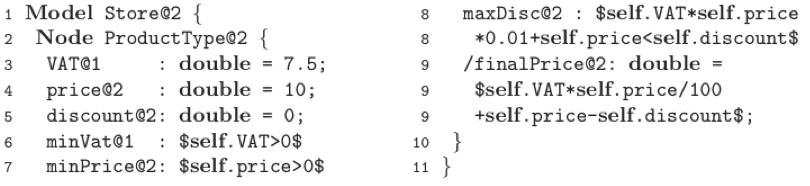
\includegraphics[width=0.9\textwidth]{images/chap3_metadepth_constraints.png}
\caption{Constraints and derived fields in Metadepth.}
\label{fig:metadepth_constraints}
\end{figure}

We have declared three constraints, on line 6, 7 and 8. An example of a derived field is given on line 9. The constraints are specified between two "\$" symbols and can be defined at the level of a clabject (as done in our example) or outside of it. The \texttt{minVat} constraint was given a potency of one, which means that it will be evaluated on the meta-level directly below. This constraint cannot access the value of fields with bigger potency, like \texttt{price}, as they may not have a value yet. The declaration of the derived field \texttt{finalPrice} is similar to a normal field, except that it is preceded by a backslash and may include fields with a lower potency.

\subsection{Controlling linguistic extensions}

Linguistic extension is interesting to permit unforeseen extensions to Domain Specific Languages spawning more than one level \cite{GenericMetaDepth}. In these languages, the top-most meta-model is usually highly generic, and linguistic extensions in lower levels could therefore be useful. Figure ~\ref{fig:ling_ext} shows an extension of our running example.

\begin{figure}[h!]
\centering
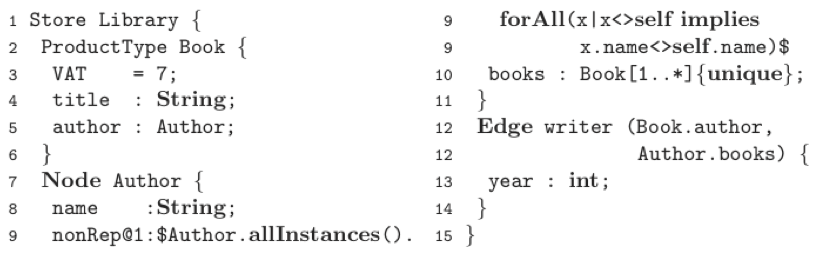
\includegraphics[width=0.9\textwidth]{images/chap3_ling_ext.png}
\caption{Linguistic extensions and associations in Metadepth.}
\label{fig:ling_ext}
\end{figure}

In the scenario above, we are interested in associating an author with \texttt{ProductType} instances. To achieve this, we linguistically extend the \texttt{Store} model by adding a new node \texttt{Author}, instance of \texttt{Node} in the linguistic meta-model (briefly discussed earlier). Authors are related to one or more books, modelled through the field books. The \texttt{\{unique\}} modifier ensures that a given \texttt{Author} is not related to the same \texttt{Book} twice.
\\ \\
Associations can be annotated with fields by explicitly defining an \texttt{Edge} between their association ends. In the example above, we have an association \texttt{writer} instantiated as an \texttt{Edge} that relates books and authors. This \texttt{Edge} has got an extra field \texttt{year} that includes the year in which the book was written by that author. We could also define a more generic type of association. We could refer to linguistic types, like \texttt{Node}, when defining association ends. This makes sense if we want to specify that a certain association end is to be taken by any (linguistic) instance of \texttt{Node}.

\section{Other deep meta-modeling solutions}

Metadepth offers one solution to the problem of deep meta-modeling. However, other solutions exist, but not all are offered as complete frameworks. For example, DeepJava \cite{LiberateProgramming} is an extension of Java with the concept of potency, thus it cannot be considered as a framework. It does provide methods with potency, but needs special keywords to navigate up the type hierarchy in order to find attribute values. The constraints and computations for derived attributes in Metadepth can access type fields in a uniform way. This approach is preferred because it has the advantage that the number of meta-levels do not matter for a given field.
\\ \\
Next to DeepJava, another proposal for deep meta-modeling has been developed \cite{MultiLevelLangEng}. This tool is largely based on \textit{Ecore}. It considers multi-level constraints and proposes extending OCL to cope with multiple ontological meta-levels. This approach is similar to MetaDepth, but MetaDepth has got the ability of assigning \textit{potency} to constraints, which makes them easier to define on multiple meta-levels. More information about these concepts can be found in \cite{MultiLevelLangEng} and \cite{MetaDepth}.

\chapter{Android Development}

Android offers a software stack for mobile devices. Apart from what people refer to as the Operation System, it also contains middleware and key applications. The Android SDK offers the necessary tools and APIs to start developing Android applications. These applications are developed using the Java programming language. The following are the most important features of the Android stack:

\begin{itemize}
\item{\textbf{Application framework} enabling reuse and replacement of components}
\item{\textbf{Dalvik virtual machine} optimized for mobile devices}
\item{\textbf{SQLite} for structured data storage}
\item{\textbf{Media support} for common audio, video, and still image formats (MPEG4, H.264, MP3, AAC, AMR, JPG, PNG, GIF)}
\item{\textbf{GSM Telephony} (hardware dependent)}
\item{\textbf{Bluetooth, EDGE, 3G, and WiFi} (hardware dependent)}
\item{\textbf{Camera, GPS, compass, and accelerometer} (hardware dependent)}
\item{\textbf{Rich development environment} including a device emulator, tools for debugging, memory and performance profiling, and a plugin for the Eclipse IDE}
\end{itemize}

\section{Android Architecture}

This section will explain the major components of the Android architecture. The complete architecture is depicted in figure ~\ref{fig:android_architecture}. We will follow a top-down approach, starting with the lowest level of abstraction (Applications) first all the way down to the Linux Kernel, that provides core system services such as security and memory management.

\begin{figure}[h!]
\centering
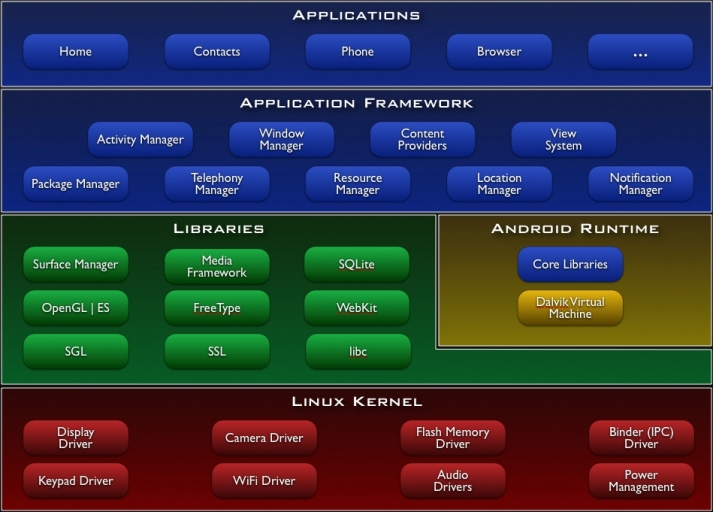
\includegraphics[width=1.0\textwidth]{images/chap4_android_architecture.jpg}
\caption{Android Architecture.}
\label{fig:android_architecture}
\end{figure}

\subsection{Applications}

Android applications are developed using the Java programming language. By default, Android ships with a number of default applications written in Java. These include an email client, SMS program, calendar, maps, browser, contacts and others. In the next section, we will see the major components of a typical Android application. In other words, the building blocks of a minimal Android application.

\subsection{Application Framework}

Android offers the ability to build extremely rich and innovative applications. Developers are granted the same access to the framework APIs used to build the core applications on the top level. The application architecture is designed to simplify the reuse of components; any application can publish its capabilities and any other application may then make use of those capabilities \cite{WhatAndroid}. 
\\ \\
Underlying all applications is a set of systems and services:

\begin{itemize}
\item{A set of \texttt{Views} to build the front-end of the application, including lists, grids, text boxes and buttons. A subset of these Views will be supported on the modeling framework.}
\item{\texttt{Content providers} that manage access to a structured set of data. They encapsulate the data, and provide mechanisms for defining data security. Content providers are the standard interface that connects data in one process with code running in another process. \cite{ContentProviders}}
\item{\texttt{Resource Manager} that provides access to non-code resources such as images and strings, so they can be maintained independently.  Externalizing your resources also allows you to provide alternative resources that support specific device configurations such as different languages or screen sizes, which becomes increasingly important as more Android-powered devices become available with different configurations. \cite{AppResources}}
\item{\texttt{Notification Manager} that notifies the user of events that happen. It allows a developer to tell the user that something has happened in the background \cite{NotificationManager}. For instance, the receival of an SMS can trigger a notification.}
\item{\texttt{Activity Manager} manages the lifecycle of one Activity. More details on Activities and the management can be found in the next section.}
\end{itemize}

\subsection{Libraries}

Although the Android SDK is offered in the Java programming language, the lower level libraries are a set of C/C++ libraries used by various components in the Android system. Like in a typical stacked architecture, a lower level layer is exposed through a higher level layer. Therefore, these libraries are accessible through the Android application framework. Some of the core libraries \cite{WhatAndroid}:

\begin{itemize}
\item{\textbf{System C library} - a BSD-derived implementation of the standard C system library (libc), tuned for embedded Linux-based devices}
\item{\textbf{LibWebCore} - a modern web browser engine which powers both the Android browser and an embeddable web view}
\item{\textbf{SGL} - the underlying 2D graphics engine}
\item{\textbf{SQLite} - a powerful and lightweight relational database engine available to all applications}
\end{itemize} 

\subsection{Android Runtime}

As seen in the above layers, Android has quite a unique application component architecture. In order to make the Android environment suitable for multiple applications, Android executes multiple instances of its own customized Virtual Machine, Dalvik. Basically, each Android application runs in its own process, with its own instance of the Dalvik Virtual Machine. 
\\ \\
As a result of this approach to multiprocessing, Android must efficiently divide memory into multiple heaps, where each heap is as small as possible, so that many applications can fit in memory at the same time. In order to be space-efficient, Android uses a special component lifecycle, which enables objects to be garbage-collected and recreated. Next to this, Dalvik is able to run a bytecode system specifically developed for Android, called dex. Dex bytecodes are approximately twice as space-efficient as Java bytecodes, halving the memory overhead of Java classes for each process.

\subsection{Linux Kernel}

Finally, Android relies on a linux kernel for core system services such as security, memory management, process management, network stack, etc. This kernel also acts as an abstraction layer between the hardware and the rest of the software stack. It controls the hardware elements throughout the software stack and serves as a gateway.

\section{Android Components}

This section will describe the different Android components and their respective managers in depth. We will start with a comparison of traditional versus Android programming. While every Android application is developed in the Java programming language, the approach of writing such an application is different from writing traditional (desktop) applications.

\subsection{Traditional versus Android programming}

When starting applications in a traditional Operating System, there usually exists a single point of entry called \texttt{main}. The OS will load the program code into a process and starts executing it. Additionally, if we look at programs written in Java, it gets a little more complex. A Java virtual machine (JVM) that resides within a process loads bytecode to instantiate Java classes as the program uses them. This process is depicted in figure ~\ref{fig:java_app}.
\\ \\
\begin{figure}[h!]
\centering
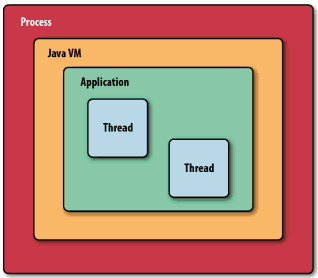
\includegraphics[width=0.5\textwidth]{images/chap4_java_app.png}
\caption{A Java application running in a JVM.}
\label{fig:java_app}
\end{figure}
The Android system works a little different and supports multiple application entry points. Instead of a sequential code hierarchy, an Android program is a cooperating group of components that may be started from outside the normal flow of the application. For example, if your application starts the activity in the camera application that captures a photo, that activity runs in the process that belongs to the camera application, not in your application's process. The photo capture function can be integrated by many applications in their UI flow.

\subsection{Activities and Intents}

Typically, an Android activity is a unit of interaction. It usually fills the whole screen of an Android mobile device. It also functions as a unit of execution. Note that an Android application does not have a single point of entry; an application can have entry points to multiple activities. They are the reusable, interchangeable parts of the flow of UI components across Android applications. An activity interacts with the Android runtime to implement key aspects of the application life cycle.
\\ \\
Now if one activity invokes another, we usually want to pass some information to it. The unit of communication is called Intent. They are the basis of a system of loose coupling that allows activities to launch one another. It is usually a bad idea to keep references to activities in memory, because of the way Android does garbage collection and the restrictions of memory on a mobile device. In general, an activity is an isolated and independent object that only communicates with other activities through intents.

\subsection{Tasks}

So communication in an Android application is defined by means of an intent. Unlike in traditional desktop applications, the UI flow in Android applications is also described through intents. Using these intents, an Android developer can create a chain of activities that spans more than one application. This is referred to as a \texttt{task}. An example of a task spanning multiple activities is depicted in figure ~\ref{fig:android_task}.

\begin{figure}[h!]
\centering
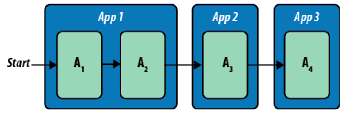
\includegraphics[width=0.7\textwidth]{images/chap4_android_task.png}
\caption{Activities in a single task spanning multiple applications.}
\label{fig:android_task}
\end{figure}

An example of this task can be found in table ~\ref{tab:table1}. In this example, app 1 represents the Android Messaging app. First, a user views all messages and after that decides to read a specific message. These two actions map onto two activities. Afterwards, he decides to view the contact, and the user is sent to another application (and another Activity). When the user decides to call this contact, we need another application again. This one task thus involved three applications and four activities. The UI flow in this task is completely defined by means of intents.

\begin{table}[h!p!]
\caption{A single task across multiple applications and spanning multiple activities}
\begin{tabular}{| l l l |}
\hline
App & Activity & User's next action \\
\hline
Messaging & View list of messages & User taps on a message in the list \\
Messaging & View a specific message & User taps Menu - View Contact \\
Contacts & View a contact & User taps Call Mobile \\
Phone & Call the contact's mobile number & nothing \\
\hline  
\end{tabular}
\label{tab:table1}
\end{table}

\subsection{Other components}

Apart from the \texttt{Activity} class, there are three other important components that contribute to Android applications: services, content providers and broadcast receivers. 
\\ \\
A \texttt{Service} class supports long-running background tasks. They may be active, but not visible on the screen. A typical application that may contain a \texttt{Service} class is a music player. We usually want to continue listening to music while doing some other task.
\\ \\
Next, a \texttt{ContentProvider} class provides access to a data store for multiple applications. An Android developer specifies a special URI starting with \texttt{content://} that gives access to the data store. A \texttt{ContentProvider} class works analogous to a RESTful web service. They have a specific URI and associated operations such as putting and getting data.
\\ \\
Finally, the \texttt{BroadcastReceiver} class allows multiple objects to listen for intents broadcast by applications. \texttt{BroadcastReceiver} is similar to \texttt{Activity}, but does not have its own user interface. 
\\ \\
While these components can possibly be important in Android applications, currently only the \texttt{Activity} class will be supported in our modeling framework. The other components can additionally be implemented as future work.

\subsection{AndroidManifest}

In order for an Android application to know what its contents are, we need to explicitly describe them in an XML file called \textit{AndroidManifest.xml}. In this file, we declare all our activities, services, content providers and broadcast receivers along with their intents. Since an Android application does not have a single point of entry, we also need to specify which component is the main component (also done through another \texttt{Intent}). A visualization of the structure of the AndroidManifest can be found in figure ~\ref{fig:android_manifest}.

\begin{figure}[h!]
\centering
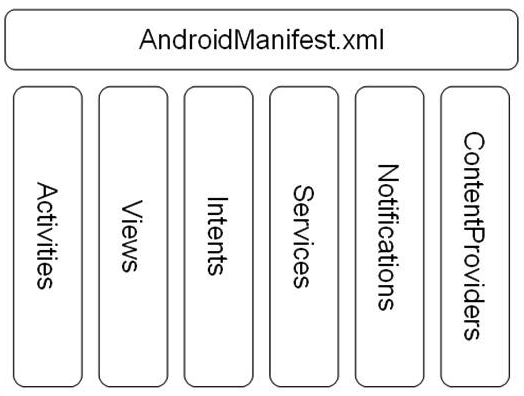
\includegraphics[width=0.7\textwidth]{images/chap4_android_manifest.png}
\caption{Structure of an AndroidManifest.xml.}
\label{fig:android_manifest}
\end{figure}

\subsection{Activity Lifecycle}

As explained earlier, the Android system can enable objects to be garbage collected and recreated. Due to this mechanism activities have a special customized life cycle, because they can easily be garbage collected when inactive. When a user wants to activate the activity again, the Android system will need to be able to recreate the \texttt{Activity} object. Activities are saved on an \textit{activity stack}. The \texttt{Activity} on top of the stack is always the running activity. Activities on the stack below the current one are always invisible and inactive. An activity can be in one of four states:

\begin{itemize}
\item{\textit{Active} or \textit{Running} if the activity is in the foreground of the screen}
\item{\textit{Paused} if the activity has lost focus but is still visible. This activity is still alive but can be killed by the Android system in case of low memory.}
\item{\textit{Stopped} if the activity is obscured by another activity. All state information is still in memory, but the activity is not visible and will most likely be killed when memory is needed elsewhere.}
\item{When the activity is \textit{paused} or \textit{stopped}, the system can ask to finish it or simply kill its process. When a user requests access to the activity again, it should be restored to its previous state.}
\end{itemize}

In figure ~\ref{fig:activity_lifecycle}, the important states of an Activity lifecycle are visualized. The states an Activity can be in are the colored ovals. The rectangles introduce the callbacks a developer can implement to perform operations when moving between states.

\begin{figure}[h!]
\centering
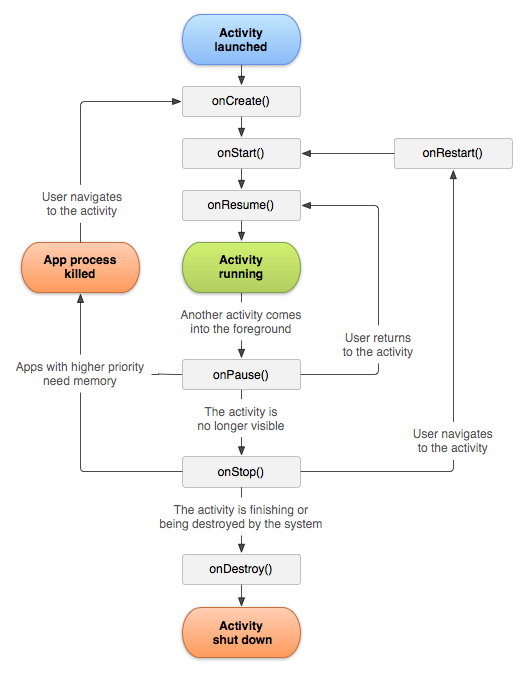
\includegraphics[width=0.9\textwidth]{images/chap4_activity_lifecycle.png}
\caption{The lifecycle of an Android Activity.}
\label{fig:activity_lifecycle}
\end{figure}

\section{Android App Inventor}

Android App Inventor is an application provided by Google that allows anyone to create applications for the Android system. Google wanted to encourage people to create software for the Android platform, even people unfamiliar with computer programming. App Inventor provides a graphical interface that has drag-and-drop functionality, so that users can easily create new applications or prototypes. An example of the application is depicted in figure ~\ref{fig:app_inventor}.

\begin{figure}[h!]
\centering
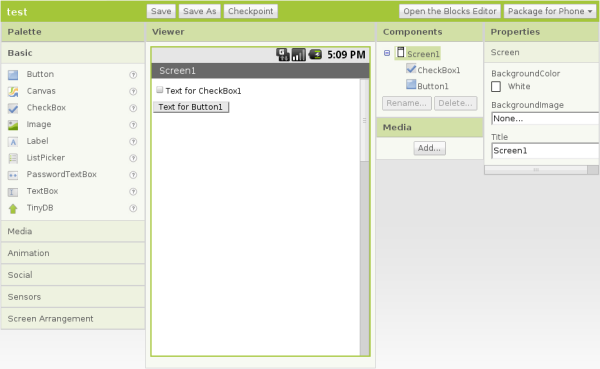
\includegraphics[width=1.0\textwidth]{images/chap4_app_inventor.png}
\caption{Google App Inventor.}
\label{fig:app_inventor}
\end{figure}

However, Google terminated the App Inventor on December 31, 2011. MIT Center for Mobile Learning is now supporting it under the name "App Inventor Edu". The Android App Inventor has been a source of inspiration in the development of my own modeling framework. 


\chapter{Collaboration}

In this chapter, we will introduce different types of collaborative methods. People will continue to interact in new and different ways. One outcome of the marriage between technology and communication is a technical workplace. The study of such workplaces gives rise to a new field: \textit{Computer-Supported Cooperative Work} (CSCW). CSCW analyzes the way groups work and seeks to discover how technology can help them work. Sometimes we refer to CSCW as \textit{groupware}. Often this term is used synonymously with CSCW technology. However, this is not completely true. In the following sections, we will define the concept of groupware and CSCW applications. We will also create a taxonomy of groupware and compare this taxonomy to CSCW applications. There exists another collaborative method, especially targeted at collaborative learning, \textit{Computer-Supported Collaborative Learning} (CSCL). This collaborative method is a refinement of CSCW. When studying these methods, we should make a clear distinction between cooperative and collaborative work. Cooperative work is accomplished by the division of labour among participants. It is an activity where each person is responsible for a portion of the problem that's being solved. Collaboration involves the mutual engagement of participants in a coordinated effort to solve the problem together \cite{DivisionCSCL}.
\\ \\
The second part of this chapter defines the collaborative patterns typically used in a collaborative application (whether it is defined as groupware, CSCW or CSCL). We finish this chapter with a collaboration stack that defines the different levels in collaborative applications.

\section{Groupware}

In the following section, we will first give a definition for Groupware. Next, we will discuss different taxonomies of Groupware and concepts of real-time (distributed) Groupware, which is the emphasis of the collaborative modeling framework. Subsequently we will discuss the benefits and drawbacks of distributed interaction, which is a central concept in distributed Groupware. Finally, we will give a classification of Groupware which states the different concepts a Groupware application should support.

\subsection{Definition}

Several definitions for groupware exist. Some define groupware as collaborative software for small focused groups, that do not give organization-wide support. Another definitions says that groupware can be viewed as the class of applications arising from the merging of computers and large information bases and communications technology. These applications may or may not specifically support cooperation. Ellis et al define groupware as follows:
\begin{mydef}
\textbf{Groupware}. computer-based systems that support groups of people engaged in a common task (or goal) and that provide an interface to a shared environment. \cite{CSCWGroupware}
\end{mydef}
In this definition, the writer uses the notions of \textit{common task} and \textit{shared environment}. This definition excludes multi-user environments where people do not share a common task. Moreover, the definition does not require users to be active at the same time. We can make a distinction between \textit{real-time groupware} and \textit{non-real-time groupware}. Our modeling framework tries to support both real-time as well as non-real-time groupware.
\\ \\
Furthermore, we can argue what distinguishes groupware from non-groupware. According to Koch, '\textit{the core characteristic of groupware is the non-separation or non-isolation of users from each other. Groupware explicitly provides awareness of the co-workers and their activities and does not separate the users from each other as it is common in distributed systems in general.}' \cite{CSCWConcepts}.

\subsection{Communication, Collaboration and Coordination}

A groupware application does not only support interactions between a user and the system. Its main strength is the interaction among users, moreover group interactions. As we focus on how to support this group interaction, we must address issues in three areas: communication, collaboration and coordination.
\\ \\
The main problem we currently stumble upon in collaborative applications is the separation of synchronous and asynchronous communication. For instance, asynchronous communication such as electronic mail and bulletin boards still exists separately from synchronous communication such as telephone or face-to-face conversations. 
\\ \\
Similar to communication, a collaborative application should support collaboration. Collaboration demands that people share information. The last years, we saw a lot of improvement on this part because of the rise of social networks such as Facebook \cite{Facebook} and purely collaborative applications such as Google Docs \cite{GDocs} or Skype \cite{Skype}. However, current information systems (such as a database system) seldom allow users to modify different parts of an object simultaneously. Usually, a user must check out this object after which it is locked for other users. Only then a user can manipulate this object. Afterwards, this user has to commit its changes again to release the lock on the object. Ideally, we need a shared environment where users are notified and updated of other's actions. 
\\ \\
Finally, if we can effectively coordinate all the actions each user performs, the effectiveness of communication and collaboration can be enhanced significantly. Coordination is a requirement in a groupware application if we want to avoid conflicting or repetitive actions between users.

\subsection{Taxonomies}

If we look at groupware, we can define a time-space separation. In terms of space, groupware can be helpful to a face-to-face group or a group that is distributed over many locations. Furthermore, the communication and collaboration can be enhanced synchronously (in real-time) or asynchronously (in non-real-time). This separation suggests four categories of groupware, as depicted by the 2x2 matrix in table ~\ref{tab:groupware_taxonomy}.
\begin{table}[h!p!]
\begin{tabular*}{0.75\textwidth}{ r | p{5cm} | p{5cm} |}
\multicolumn{1}{r}{}
 &  \multicolumn{1}{c}{Same Time}
 & \multicolumn{1}{c}{Different Times} \\
\cline{2-3}
Same Place & face-to-face interaction & asynchronous interaction \\
\cline{2-3}
Different Places & synchronous distributed interaction & asynchronous distributed interaction \\
\cline{2-3}
\end{tabular*}
\caption{Groupware 2x2 Time Space Matrix}
\label{tab:groupware_taxonomy}
\end{table}
\\
For instance, meeting room technology would belong to the upper left cell, a real-time document editor within the lower left cell, a physical bulletin board within the upper right cell and an electronic mail system within the lower right cell. Our modeling framework allows the generation of applications that support both synchronous and asynchronous distributed interaction. 
\\ \\
This taxonomy can be extended by the fact that our activities can be predictable or unpredictable \cite{CSCLHistory2}. The extended taxonomy is shown in figure ~\ref{fig:ext_taxonomy}.
\begin{figure}[h!]
\centering
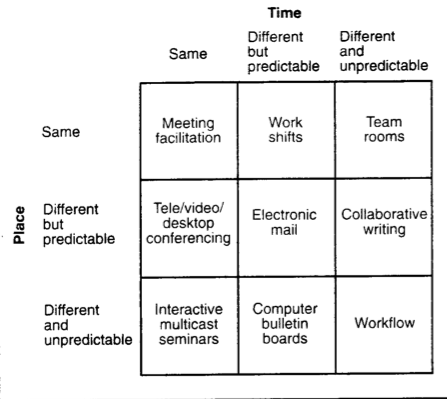
\includegraphics[width=0.7\textwidth]{images/chap5_3by3matrix.png}
\caption{Groupware 3x3 Time Space Matrix}
\label{fig:ext_taxonomy}
\end{figure}
Activity can be carried out in a single place (top row), in several places known to the participants (middle row) or in numerous places, not all of which are known to the participants (bottom row). Each of these activities can then be carried out in real time (left column), at different times that are highly predictable (like sending a mail to a colleague and expecting it to be read within a day) or at different times that are unpredictable (like collaborative writing).

\subsection{Real-time Groupware Concepts}

The concept of groupware is not new. It has been around since the early nineties, but it is still constantly evolving. In this section, we define some important terms for comparing groupware systems. These concepts will mainly be applicable on real-time groupware. In the remainder of this chapter we will also mainly focus on real-time applications, because they are mainly used for easy and effective communication and collaboration.

\begin{itemize}
\item{\textit{Shared context}. A shared context is a set of objects where the objects and the actions performed on the objects are visible to a set of users. For example, a group of users can make notes on files shared in a Dropbox shared folder or class notes within electronic classrooms.}
\item{\textit{View}. A view is a representation of some portion of a shared context. Different views might display the same information in different ways or they can use the same presentation but refer to different parts of the shared context. For example, we can show a dropbox folder as a list of filenames or as a group of images showing an in-file view.}
\item{\textit{Synchronous and asynchronous interaction}. Synchronous interaction happens when people interact in real-time and asynchronous action happens when people interact over an extended period of time. Usually, a groupware application only supports one of the two interaction types. Our modeling framework allows the creation of both interaction types at the same time.}
\item{\textit{Session}. A session usually represents a period of synchronous interaction supported by a groupware system. When a user logs in into a groupware system, he starts his session and can start interacting with other users that currently own a session.}
\item{\textit{Role}. A role is a set of privileges or responsibilities related to a user. For instance, a user can be assigned the role of admin to control a groupware application.}
\end{itemize}

\subsection{Benefits and drawbacks of distributed interaction}

If we look at the taxonomy of groupware systems and only consider systems at different places, we get a distributed interaction model. From a user's perspective, these distributed interaction sessions are completely different experiences from face-to-face (i.e. same place) sessions. Because our modeling framework primarily targets interaction at different places, we list the benefits and drawbacks of these distributed interaction types here: 

\begin{itemize}
\item{\textit{Encourages parallel work within the group}. Usually, people divide into subgroups to work on different parts of an assignment. It is easy for distributed members to drop out for a while, do something else and then return. In most face-to-face situations, this is not socially acceptable.}
\item{\textit{Increases information access}. Apart from sources on the internet, participants in distributed sessions have access to local books and files.}
\item{\textit{Makes discussion more difficult}. In comparison to face-to-face sessions, it is a lot harder to have a discussion or host a panel over a distributed session. Usually, people tend to take turns and are unusually polite.}
\item{\textit{Cuts down on social interaction}. This item has both a positive and a negative connotation. Distributed sessions are usually more serious. As a consequence, there is less interchange about nontask-related topics and people tend to focus on the task immediately. The effect is a possible efficiency gain from time saved and a possible loss from social needs.}
\item{\textit{Can be efficient}. Distributed sessions allow for parallel work. In contrast to face-to-face sessions, people in a distributed session are usually more concentrated on the to be accomplished task itself.}
\end{itemize}

\subsection{A groupware classification}

Groupware is about crewing computer-based systems that support groups of people involved in a common task. This is a very open definition and in practice it is often hard to decide what kind of functionality a particular group needs. In general, we can distinguish five application classes:

\begin{itemize}
\item{\textbf{Awareness support} - This class is one of the core concepts in groupware. Groupware tries to connect people and allows to coordinate each other. Almost every groupware application has some sort of Awareness support.}
\item{\textbf{Communication support} - In order for people to be connecting with each other, we need some sort of communication in the groupware system. This sort of communication can be of a synchronous or asynchronous nature. Asynchronous communication examples are email or forums. Synchronous communication examples are chat or video.}
\item{\textbf{Coordination support} - There is already some contribution to coordination through awareness, but in a very general way. We might need explicit coordination support in the form of workflow solutions.}
\item{\textbf{Team support} - Not every person in a group of people will have the same needs and abilities within a groupware application. There is a need for special group types and their special needs. We might need to define roles that allow people to do different things within the application.}
\item{\textbf{Community support} - Teams and communities are a different thing. To begin with, they have a different structure and probably completely different needs. A team is a group of people usually working on a bigger cause or goal. A community often does not consist of equals working together on the same things. There are many different functions in a community that make the groupware application complex.}
\end{itemize}

When we are faced with a particular situation, it is quite straightforward to identify one or two classes that cover the requirements in this situation. From there on, we can select the appropriate tools to start building the groupware application.

\section{Computer-Supported Cooperative Work}

Like groupware, CSCW is concerned with understanding social interaction and the design, development and evaluation of technical systems supporting social interaction in teams and communities. It researches the use of computer-based technology for supporting collaboration. In this section, we will define CSCW exactly, look at a few design challenges and study the technology behind CSCW.

\subsection{Definition}

Many researchers in CSCW have their own definition of what CSCW exactly is. Bowers and Benford have the most general sight: '\textit{In its most general form, CSCW examines the possibilities and effects of technological support for humans involved in collaborative group communication and work processes}' \cite{StudyCSCW}. Greif defines CSCW as '\textit{computer-assisted coordinated activity such as communication and problem solving carried out by a group of collaborating individuals.}' \cite{CSCWReadings}. Wilson on his turn defines CSCW as '\textit{a generic term which combines the understanding of the way people work in groups with the enabling technologies of computer networking, and associated hardware, software, services and techniques}' \cite{CSCWIntro}. In general, we can make a distinction between the social and technological definition of CSCW. The following CSCW definitions are the most appropriate definitions for what we have in mind.
\begin{mydef}
\textbf{CSCW: Social Definition}. CSCW should be conceived as an endeavor to understand the nature and characteristics of cooperative work with the objective of designing adequate computer-based technologies. \cite{CSCWChars}
\end{mydef}
\begin{mydef}
\textbf{CSCW: Technological Defintion}. computer-based systems that support groups of people engaged in a common task (or goal) and that provide an interface to a shared environment. \cite{CSCWGroupware}
\end{mydef}
Note that the technological definition of CSCW is the same as that one of Groupware. The exact difference between CSCW and Groupware will be explained in the next subsection.

\subsection{CSCW is Groupware}

CSCW is an interdisciplinary field where researchers from various fields contribute with '\textit{different perspectives and methodologies for acquiring knowledge of group work and for suggesting how the group's work could be supported}' \cite{CSCWGroupware}. For instance, '\textit{computer scientists might bring in their technical knowledge and social scientists contribute their sociological and anthropologistic knowledge for questions of design}' \cite{CSCWMethodology}.
\\ \\
How does all of this relate to Groupware? In general, groupware is the term coined for the technical system resulting from CSCW research and development. Groupware is the technical part of the CSCW system. Moreover, many software systems that have collaborative functionality will be groupware to some extent. However, CSCW as a research field will persist, because it addresses larger questions about the design and refinement of groupware \cite{CSCWReadings}.

\subsection{Challenges in CSCW design}

CSCW is not a typical software design activity. Several authors in the field have been analyzing CSCW projects and have been identifying core challenges of collaborative system design compared to software design in general \cite{CSCWConcepts}. 

\begin{itemize}
\item{It is hard to capture the requirements for a collaborative system, because the requirements are not clearly known to all participants or they change over time.}
\item{All of the potential users have to use the CSCW system actively in order for the system to be a success.}
\end{itemize}

In the next subsection, we will address the requirements engineering of groupware in more detail. The other challenge, the adoption of a collaborative system, is largely due to a network effect and cannot be easily manipulated.

\subsection{Requirements engineering in CSCW}

When a CSCW project was developed in the future, more often than not it was not able to satisfy its intended goals. The main reason for this problem is that most of these systems have been regarded as a technical system only. However, as we have seen there are two aspects of CSCW, a social and technological aspect. It turned out that very often the social aspect was not satisfied in the CSCW system and it was not seen as a socio-technical system. The fact that the success of such a system depends on the social group that is using it is overlooked. This fact results in several problems:

\begin{itemize}
\item{It is hard to get the requirements from users. The social group using the end-product might change and thereby changing the requirements.}
\item{When designing a CSCW system, there should be both a technical and a social design.}
\item{It might be hard to get the potential users to accept the resulting CSCW system.}
\end{itemize}

The first problem of capturing the requirements from users in an initial development phase is a known problem in software engineering. To address this issue, iterative development has been introduced. If we build a prototype that engages users and produces some feedback, we might be able to create a much better product even from one iteration more.
\\ \\
If we look at typical collaborative applications today, we notice the trend that functionalities are offered as separate applications. In order to make collaboration a true success in an enterprise, there is a need to integrate the different functionalities and to adapt applications to the need of the individual and the group. There is a need for an all-in-one collaborative applications. This is one of the issues our modeling framework tries to tackle. 

\section{Computer-Supported Collaborative Learning}

Computer-supported collaborative learning (CSCL) has some interfaces with CSCW and Groupware, but is fundamentally different in a few aspects. The focus in CSCL is on learning, as the name suggests. It is concerned with studying how people can learn together with the help of computers \cite{CSCLHistory}. In this chapter, we will see several definitions for collaboration in the context of learning. It will become clear that the interplay of learning with technology turns out to be quite intricate. 

\subsection{Education and CSCL}

Computers have become an important artifact in formal education (e.g. high school or college) as well as informal education (e.g. museums). In the broader learning sciences, there also exists a trend in learning together in small groups. However, the ability to enhance learning through technology and education remains a challenge that CSCL is designed to address. 
\\ \\
CSCL proposes the development of new software that bring learners together and that can offer creative activities of intellectual exploration and social interaction. It is often conflated with e-learning, the organization of instruction across computer networks. E-learning is often associated with the creation and delivery of digital content such as slides, text or videos. There are a few problems with this view:

\begin{itemize}
\item{Digital content such as slides, text or videos does not necessarily make for compelling instruction. It may provide important resources for students, but there must exist a larger interactive context.}
\item{Online teaching requires as much effort by human teachers as classroom teaching.}
\item{CSCL stresses collaboration among the students, so that they are not simply reacting in isolation to posted materials.}
\item{CSCL is concerned with Face-to-Face collaboration, either synchronously or asynchronously.}
\end{itemize}

\subsection{Definition}

Even more than in groupware, a distinction between cooperation and collaboration is conceptually central in this review of CSCL. Cooperative work is accomplished by the division of labour among participants. It is an activity where each person is responsible for a portion of the problem solving. Collaboration involves the mutual engagement of participants in a coordinated effort to solve the problem together.
\\ \\
Before CSCL became a research topic, there had been a lot of research conducted on group learning. To distinguish CSCL from group learning, we can draw a distinction between \textit{cooperative} and \textit{collaborative} learning:

\begin{mydef}
In cooperation, partners split the work, solve sub-tasks individually and then assemble the partial results into the final output. In collaboration, partners do the work 'together' \cite {DefinitionCSCL}.
\end{mydef}

In cooperation, the learning is done by individuals who contribute their results and present these as their group product. Cooperative learning in groups is an activity that takes place individually. In contrast, collaborative learning occurs socially as the collaborative construction of knowledge. The activities that individuals engage in are not individual-learning activities, but group interactions like negotiation and sharing.
\\ \\
Finally, a formal, programmatic definition of CSCL was presented by Koschmann \cite{DefinitionCSCL2}:
\begin{mydef}
CSCL is a field of study centrally concerned with meaning and the practices of meaning-making the context of joint activity, and the ways in which these practices are mediated through designed artifacts.
\end{mydef}
"Practices of meaning-making in the context of joint activity" might be hard to understand. It means that learning is not merely accomplished through interaction, but it is \textit{constituted} of interactions between participants. 

\section{Collaborative Patterns}

In the previous sections we have discussed the different kinds of collaborative applications. In general, we may conclude that a collaborative application provides a group of users with the facility to communicate and share data in a coordinate way. In this section, we will propose several design patterns to help in the design and development of collaborative applications. These patterns cover the basic aspects such as data sharing and communication.
\\ \\
Every pattern proposed will describe a \textit{context} within which we can use this pattern, the \textit{problem} the pattern solves and the \textit{solution}. We will describe the \textit{forces}, \textit{implementation}, \textit{examples} and \textit{related patterns} as well. All these individual patterns can be interwoven into a \textit{patterns system} that describes how these patterns are connected, how they complement one another and how software development with patterns is supported \cite{DesignPatternsColl}. If we combine the following patterns, we arrive at a patterns system. I implemented the following patterns that form the patterns system as closely as possible in the modeling framework.

\subsection{Session}

In all collaborative applications, we have users working together in a session. A session can be both synchronous (at the same time) or asynchronous (at different times). Therefore, a session is usually tracked and we can identify who is currently connected in this session.
\\ \\
\textbf{Problem}
\\
How do we manage and coordinate a session in a collaborative application?
\\ \\
\textbf{Requirements}
\begin{itemize}
\item{Users work in groups}
\item{We need to know which users are connected and working synchronously}
\item{Data is protected from users outside of the session}
\item{It is possible to register new users}
\item{It is possible to unregister new users}
\item{We need to check a user's credentials when creating a session}
\end{itemize}
\textbf{Solution}
\\
Register a list of all users belonging to the session and show a list of users currently working and connected to the session.
\\ \\
\textbf{Examples}
\\
The collaborative modeling framework allows a developer to model a session that persists users and keeps track of currently connected users.

\subsection{Repository}

In all collaborative applications we need to store and share data.
\\ \\
\textbf{Problem}
\\
How can we provide tools to users currently connected in the session that allow them to get recourses that have been created? How can users share their own resources?
\\ \\
\textbf{Requirements}
\begin{itemize}
\item{Ability to store data}
\item{Possibility to share data}
\item{Edit or remove data that belongs to the repository}
\end{itemize}
\textbf{Solution}
\\
Provide a repository that can be managed and controls access to users.
\\ \\
\textbf{Examples}
\\
In the collaborative modeling framework, Dropbox is used as a repository. Users may upload new resources to Dropbox and a developer may model a view that shows the Dropbox repository.

\subsection{Object}

Every object (e.g. chat message, dropbox resource, generic list) that is created should be saved in order to provide data awareness. We typically save the meta-data related to the object, such as the user, the object type and the time.
\\ \\
\textbf{Problem}
\\
Data is generated by the members of a workgroup. How can we manage this data?
\\ \\
\textbf{Requirements}
\begin{itemize}
\item{Users can create new objects/resources}
%\item{If we want to store multiple revisions of a file, we need to store modified objects and make them available to users}
\end{itemize}
\textbf{Solution}
\\
Provide a meta-data information object for each data object. We typically store an object's creation data and time, the user and the object type.
\\ \\
\textbf{Examples}
\\
In the collaborative modeling framework, a developer can model and include a MongoDB \cite{MongoDB} database to persist all in-app objects and their meta-data. 

\subsection{View}

In a collaborative application, it is necessary to have a graphical view of the repository's data. Various groups of users may have various views.
\\ \\
\textbf{Problem}
\\
How can we provide a view of the data in the repository?
\\ \\
\textbf{Requirements}
\begin{itemize}
\item{All users should have access to the data they have created}
\item{Some data needs to be hidden from certain users}
\end{itemize}
\textbf{Solution}
\\
Users are able to view the data in the repository, optionally in different views.
\\ \\
\textbf{Examples}
\\
In the collaborative modeling framework, it is currently only possible to view the repository's resources in a list view. In the future, multiple views might be supported. The repository might show both the resource itself as well as its meta-data.

\subsection{Broadcast}

A user typically wants to send or share objects with other users in a session. Depending on the object type, a user may be able to send the object to all connected users, to all users or to a group of users.
\\ \\
\textbf{Problem}
\\
How can we send objects to other users?
\\ \\
\textbf{Requirements}
\begin{itemize}
\item{Users can send an object to a single connected user}
\item{Users can send an object to all connected users}
\item{Users can send an object to all users (connected or disconnected)}
\end{itemize}
\textbf{Solution}
\\
We need a broadcast technique to send objects to other users. This is a technical detail discussed in the next chapter.
\\ \\
\textbf{Examples}
\\
In the collaborative modeling framework, it is possible to model a chatroom and allow users to send messages to each other. Messages are persisted within MongoDB, so other users don't have to be connected at the time of sending the message. Currently it is not possible to send arbitrary binary data, but only text.

\subsection{User}

A user is an object that identifies a person in a group. Certain personal information about each user has to be saved. 
\\ \\
\textbf{Problem}
\\
How can we manage information about users?
\\ \\
\textbf{Requirements}
\begin{itemize}
\item{User awareness is needed in applications, so we need to keep track of certain information about each user}
\end{itemize}
\textbf{Solution}
\\
A user object contains all necessary personal information for a person to initiate a session and participate in the application.
\\ \\
\textbf{Examples}
\\
In the collaborative modeling framework, in order to participate in a session, a developer can require every user to log in with a username and a password. The developer can model these accounts and restrict public access. In order to provide user awareness, every application also display all users currently connected.

\subsection{Role}

In a collaborative application, we may have different access rights for groups of users.
\\ \\
\textbf{Problem}
\\
How can we manage the access rights of users? Not all users will have the same permissions within a collaborative application.
\\ \\
\textbf{Requirements}
\begin{itemize}
\item{Collaborative applications have different types of users}
\item{Roles are used to restrict data access}
\item{Some views can be restricted by roles}
\end{itemize}
\textbf{Solution}
\\
We assign roles to each user in order to define their rights and permissions.
\\ \\
\textbf{Examples}
\\
In the collaborative modeling framework, we can restrict access to certain objects with different user roles. For instance, we can model a list that asks questions to a user, but only a user with the admin role can see the answers. 

\subsection{Environment}

A collaborative application may contain multiple sessions, with users working on different repositories. This means that some groups might not interfere with others, in which way we can re-use an application.
\\ \\
\textbf{Problem}
\\
How can we provide access to collaborative applications with users identified among corresponding sessions? How can we control the 'environment'?
\\ \\
\textbf{Requirements}
\begin{itemize}
\item{A session member's work should not interfere with another session member}
\item{All users among the sessions should have a uniform way to enter a collaborative application}
\end{itemize}
\textbf{Solution}
\\
The \textit{Environment} object has information on all sessions of users connected to the collaborative application.
\\ \\
\textbf{Examples}
\\
In the collaborative modeling framework, a developer may model a server that maintains an environment. This \textit{server}/\textit{environment} object pertains all sessions and handles calls between client and server.

\subsection{Pattern System for Collaborative Applications Design}

All these previous patterns together define a pattern system for the design of collaborative applications. The overall system design through these patterns is depicted in figure ~\ref{fig:pattern_system}.
\begin{figure}[h!]
\centering
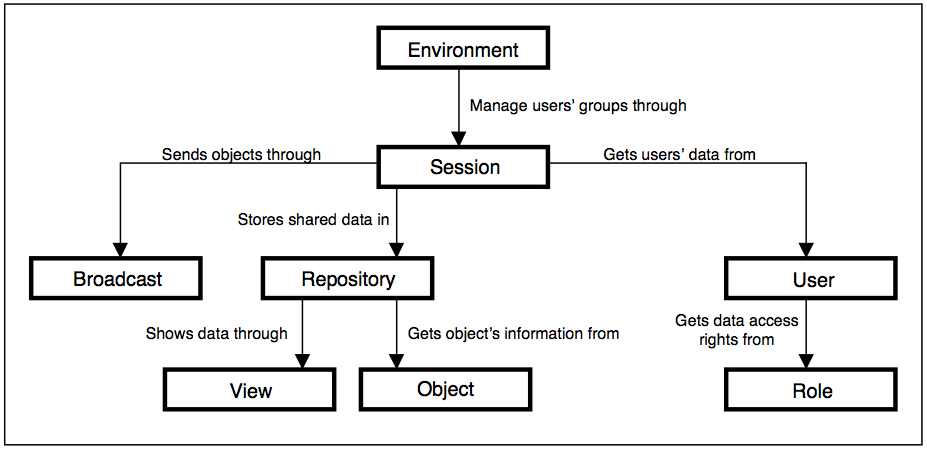
\includegraphics[width=1.0\textwidth]{images/chap5_pattern_system.png}
\caption{Pattern system of a collaborative system}
\label{fig:pattern_system}
\end{figure} \\
The environment object keeps track of all sessions in a collaborative application. A session can broadcast objects and is persisted through a user with a specific role. Furthermore, we have a Repository that is accessed through the session object and shown through a View.

\section{Collaboration Stack}

As we have seen in previous section, we have mapped the collaborative modeling framework onto the collaborative pattern system through several design patterns. These collaborative patterns can also be regarded as a kind of documentation for a proven solution \cite{CollOntology}. In this section we will present an approach for creating an ontology of collaboration patterns and patterns languages. This ontology corresponds to a "collaboration stack" that identifies the various levels of abstraction. On one side we have some abstract collaboration patterns and on the other side we have the technologies that allow these patterns to be implemented. The goal of this ontology is to see where our underlying patterns, seen in previous section, belong in a stack. All patterns described correspond with the so-called low-level collaboration patterns in the collaboration stack. We can even combine those patterns to form higher level patterns. For instance, we could combine a revision history concept with the object pattern, which would result in a higher level version control pattern. Using these patterns in an application results in a further specialization that creates collaboration services, such as a shared whiteboard.

\subsection{Ontology of collaboration patterns}

The collaboration stack is depicted in figure ~\ref{fig:coll_stack}. This stack was inspired by a typical IT protocol stack. Here we see the relation of collaboration patterns to collaborative services and their technologies. 
\begin{figure}[h!]
\centering
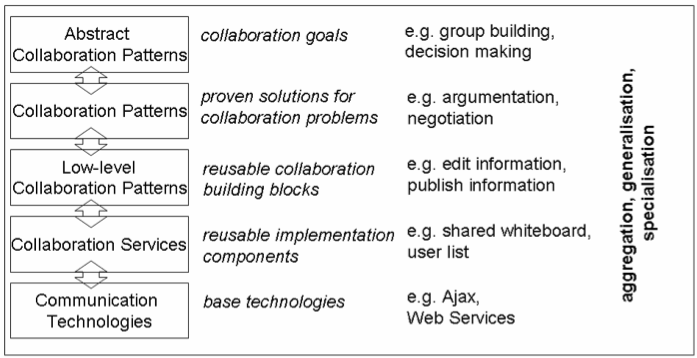
\includegraphics[width=0.9\textwidth]{images/chap5_coll_stack.png}
\caption{Collaboration Stack}
\label{fig:coll_stack}
\end{figure} \\ \\
These collaboration patterns make use of their underlying services. For instance our environment pattern from the previous section makes use of the user list to handle sessions. In turn, these collaboration services make use of basic technologies. Now that we have a clear idea of our pattern system and the corresponding collaboration stack, we can describe the design of our collaborative framework. All components and their design will be described in the next chapter.

\section{Conclusion}

Problems tackled in the framework:

-> Pattern System allows for structured solution
-> Easy to create all patterns
-> Meta-models for several components

===> Rapid validation of an idea/prototype, Ability to create an all-in-one integrated collaborative solution

\chapter{Designing a Collaborative Modeling Framework}

In this chapter, the collaborative modeling framework will be explained in depth. The target platform for applications modeled through the framework is Android. Once a modeler has a basic understanding of how Android development works, the modeler can use this framework to rapidly develop Android collaborative prototype applications. In the first section, we will give an overview of all the formalisms and technologies used in the form of a Megamodel. Next, we will describe the basic building blocks of the framework through a class diagram and discuss the meta-models that make up the core of an Android application. In the third section we describe the server component, written in Node.js \cite{NodeJS} and Javascript. The server component is used to persist data created by a user and to distributed this data to other users currently involved in a session. Finally, we end the chapter with a section on code generation and EGL \cite{EGL}.

\section{Megamodel}

Modeling-in-the-large, or \textit{Megamodeling}, considers the global relationships between models, meta-models and all formalisms used in general. In \cite{Megamodeling}, Favre describes the concept of Megamodeling as follows:
\begin{quotation}
For instance for a model to be useful, one needs a metamodel but also transformations that operates on it, and then transformation engines to interpret the transformation models, interpreters to interpret the language in which the transformation engines are written in, and so on. A megamodel is a model that represents this kind of complex arrangements without entering into the details of each artefact.
\end{quotation}
In this section, we will give an overview of all the artifacts used in the design and implementation of this work. This megamodel is depicted in figure ~\ref{fig:megamodel}.
\begin{figure}[h!]
\centering
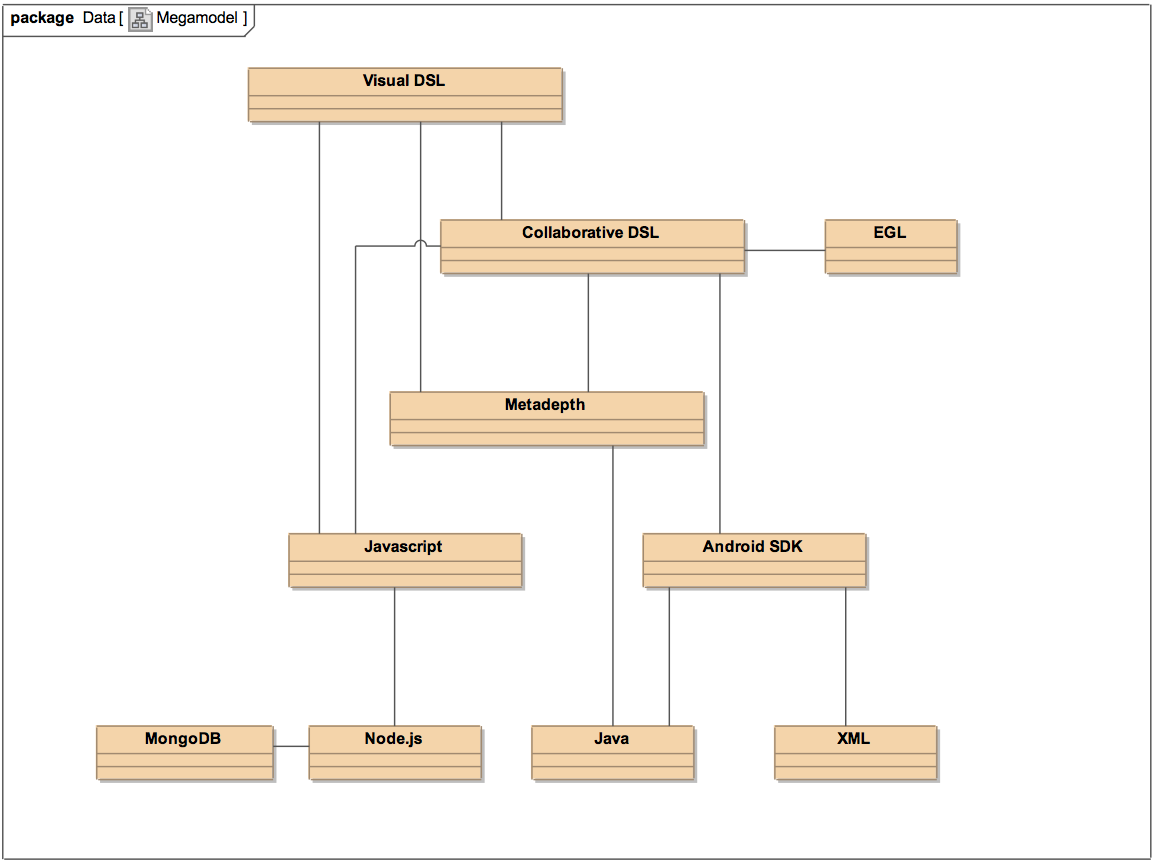
\includegraphics[width=1.02\textwidth]{images/chap6_megamodel.png}
\caption{Megamodel.}
\label{fig:megamodel}
\end{figure} \\
On the lowest levels we see all the technologies used in this work, such as Javascript, Java and XML.  On the highest level, we see the Visual DSL (see Appendix A) that uses both Javascript (to generate the visual environment itself), Metadepth (to define the meta-models) and the collaborative DSL (to provide a target mapping for a model transformation). The lines between the formalisms describe associations. For instance, the collaborative modeling framework (which is the DSL and all the build tools) uses the Android SDK, Metadepth and Javascript to build its DSL.

\section{Main component Meta-models}

In this section, we will discuss the main component meta-models featured in the collaborative modeling framework. First, a high-level overview in the form of a class diagram will be given. Next, individual meta-models will be explained in more detail.

\subsection{High-level class diagram}

In figure ~\ref{fig:highlevel_mm}, we see a high-level overview class diagram. This class diagram contains all the important meta-models that make up an application model in the framework. There is one important piece missing in the class diagram, which is the \texttt{Component} hierarchy. This hierarchy will be reviewed in section 6.3. The meta-models \texttt{Application}, \texttt{Manifest}, \texttt{Activity}, \texttt{AndroidAction}, \texttt{UIAction} and \texttt{Server} will be explained in detail in this chapter. 
\begin{figure}[h!]
\centering
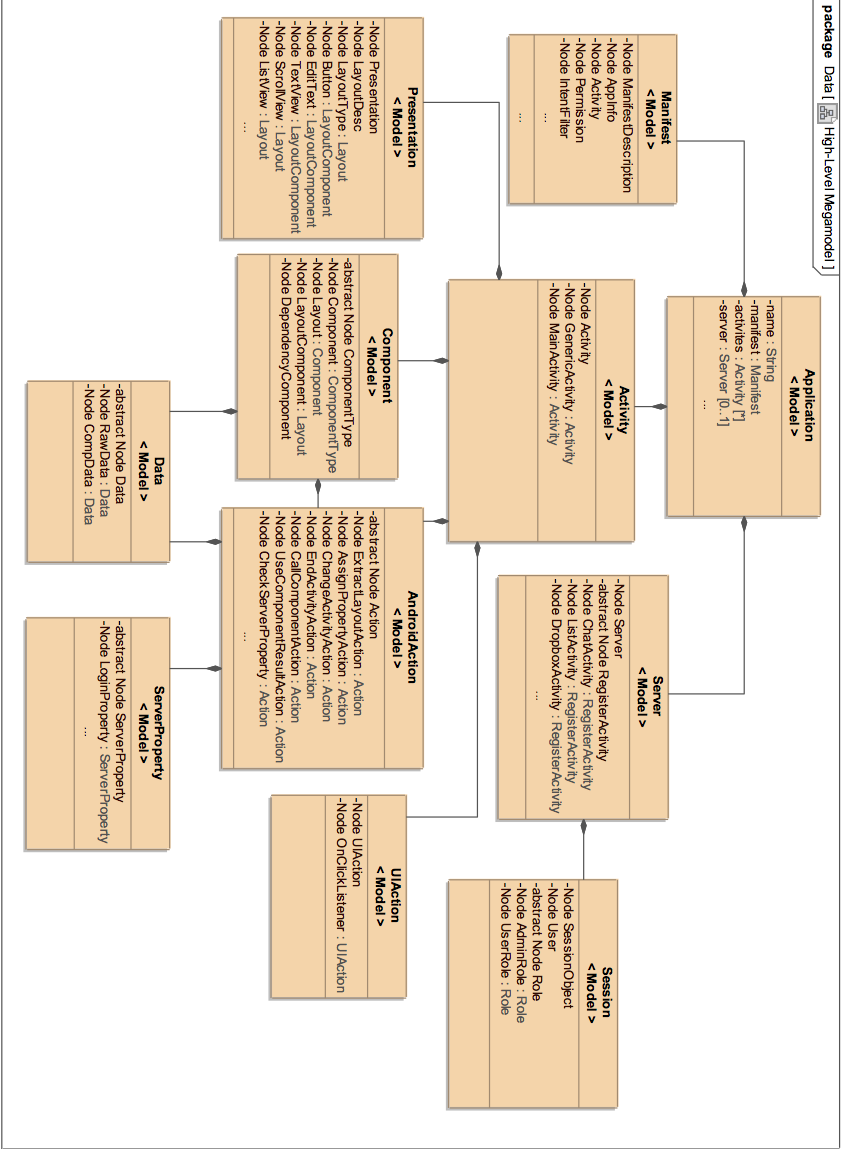
\includegraphics[width=1.02\textwidth]{images/chap6_high_level.png}
\caption{High-level Class Diagram.}
\label{fig:highlevel_mm}
\end{figure}

\subsection{Application}

The top-level meta-model that represents an Android application is the \texttt{Application} meta-model. \texttt{Application} has a \texttt{name} field and contains an \texttt{AndroidManifest} and a set of \texttt{Activities}. If we want to communicate with a server, we also need to specify an instance of the \texttt{Server} meta-model. The complete \texttt{Application} meta-model is described as follows:

\begin{lstlisting}[label=application-mm,caption=Application meta-model, captionpos=t]
load "Manifest"
load "Activity"
load "Server"

Model Application imports Activity, Manifest, Server {
	name			: String;
	manifest		: ManifestDescription[1];
	activities		: Activity[*];
	server 			: Server[0..1];
}
\end{lstlisting}

\subsection{Manifest}

One field in the \texttt{Application} meta-model is the \texttt{AndroidManifest}. The \textit{AndroidManifest.xml}, as described in chapter 4, contains all activities and other Android components. The equivalent meta-model is declared as follows:

\begin{lstlisting}[label=application-mm,caption=Manifest meta-model, captionpos=t]
Model Manifest {

	Node ManifestDescription {
		namespace		: String="http://schemas.android.com/apk/res/android";
		package			: String;
		versionCode		: String="1";
		versionName		: String="1.0";
		sdk				: String;
		app_info		: AppInfo[1];
		permissions		: Permission[*];
	}

	Node AppInfo {
		icon 		: String="@drawable/icon";
		label		: String="@string/app_name";

		activities	: Activity[*];
	}

	// e.g. <uses-permission android:name="android.permission.SEND_SMS"/>
	Node Permission {
		name 	: String;
	}

	Node Activity {
		name 	: String;
		label 	: String="@string/app_name";
		intent	: IntentFilter;
	}

	// e.g. http://developer.android.com/guide/topics/intents/intents-filters.html
	Node IntentFilter {
		action 		: String="android.intent.action.MAIN";
		category	: String="android.intent.category.LAUNCHER";
	}
}
\end{lstlisting}
Some of the fields have a pre-defined value, such as \texttt{namespace}, \texttt{icon} or \texttt{label}. Other fields need to be set explicitly by the modeler. The \texttt{package} field describes the Java package used to logically organize the source code. Other fields describe the current SDK version of Android and the Activities that correspond with the ones that are modeled in the \texttt{Activity} meta-model. The \texttt{Permission} Node models the permissions that the modeled application needs. For instance, if the application needs to access the internet, we need to add an INTERNET permission. Every Android application can have a variety of permissions set to use the functionality provided by the SDK \cite{AndroidPermissions}. An \texttt{IntentFilter} is associated to an Activity, we indicate that this Activity is the entry point of the application. In Android, other options can be specified through intent filters \cite{AndroidIntentFilter}, but these are not supported in the collaborative modeling framework.

\subsection{Activity}

The most important part of the collaborative framework is the \texttt{Activity} meta-model. It encapsulates all Android components, the layout and all actions on (layout) components. The \texttt{Activity} meta-model is designed as follows:

\begin{lstlisting}[label=activity-mm,caption=Activity meta-model, captionpos=t]
load "Presentation"
load "Component"
load "AndroidAction"
load "UIAction"

Model Activity imports Presentation, Component, AndroidAction, UIAction {

	Node Activity {
		name				: String;
		// Is this the main activity that is launched when launching the application?
		main 				: boolean;

		content				: Component@0[*];
		presentation		: Presentation[1];
		onClickListeners 	: UIAction[*];
	}

}
\end{lstlisting}
As we can see, an Activity contains an arbitrary number of components (explained in next section), a presentation model and a set of UI actions. Both the \texttt{Presentation} and \texttt{Action}/\texttt{UIAction} meta-models will be explained in next subsections.

\subsection{Presentation}

In this section, we will review the \texttt{Presentation} meta-model. This meta-model represents a mapping from the Metadepth syntax to the XML representation in Android. The \texttt{Presentation} meta-model is described in Listing ~\ref{presentation-mm}
%In an Android application, the layout of an Activity is usually presented through an XML file. Alternatively, the layout of an \texttt{Activity} can also be described through Java code. For the collaborative modeling framework, the XML approach was chosen, so the code generation part will generate a set of XML files that represent the application's layout.

\begin{lstlisting}[label=presentation-mm,caption=Presentation meta-model, captionpos=t]
load "Component"

Model Presentation imports Component {
	
	Node Presentation {
		activityname 	: String;
		layout 			: LayoutDesc[1];
	}

	Node LayoutDesc {
		name			: String;
		layoutType		: LayoutType[1];
	}

	// e.g. LinearLayout
	Node LayoutType : Layout {
		name 		: String;
		namespace	: String="http://schemas.android.com/apk/res/android";
		orientation	: String;
		width		: String="fill_parent";
		height		: String="fill_parent";

		children 	: Layout@0[*];
	}

	Node Button : LayoutComponent { }

	Node EditText : LayoutComponent {
		password 		: String;
		requestFocus	: boolean;
	}

	Node TextView : LayoutComponent { }

	Node ScrollView : Layout {
		width 		: String;
		height 		: String;
		weight 		: String;
		components 	: Layout@0[*];
	}

	Node ListView : Layout {
		width		: String;
		height		: String;
		weight		: String;
	}
}
\end{lstlisting}
The relevant part of the meta-model is defined through the \texttt{LayoutType} node. This node describes the type of layout (e.g. LinearLayout, a layout that arranges its children in a single row or column \cite{AndroidLinearLayout}) to use in the \texttt{Activity}. Apart from the type, it also contains a description of the elements contained in the layout itself. We usually want to create a \texttt{LinearLayout} type, but other types are possible too \cite{AndroidLayoutType}. Examples of layout elements are \texttt{Button} or a child view that has its own layout elements, for example a \texttt{ScrollView}.

\subsection{Action}

The \texttt{Action} meta-model is an important part in the functionality of the collaborative modeling framework. It provides a skeleton for executing actions on Android components or elements in a layout. Another example of an action would be the exchange of data between activities. A part of the \texttt{Action} meta-model is displayed in listing ~\ref{androidaction-mm}.

\begin{lstlisting}[label=androidaction-mm,caption=AndroidAction meta-model, captionpos=t]
load "Component"
load "ServerProperty"
load "Data"

Model AndroidAction imports Component, ServerProperty, Data {
	
	abstract Node Action {
		ctype			: String{id};
		condition 		: Action;
	}

	// e.g. use the value of a text field to call the action method of a component
	Node ExtractLayoutAction : Action {
		source 			: Component@0;
		name 			: String;
	}

	// Specify the target activity
	Node ChangeActivityAction : Action {
		oldActivity 	: String;
		newActivity 	: String;
		data 			: Data[*];
	}

	// Call the action method of a component.
	// Might save a value if it's a sensor (i.e. geo)
	// Or execute a real action if it's an actuator (i.e. send an SMS)
	Node CallComponentAction : Action {
		// properties needed to call the action method of the component
		properties		: Data[*];
	}
}
\end{lstlisting}
The actions listed above are the three most used and important actions. The \texttt{ExtractLayoutAction} takes as arguments a source layout component and a name for the data that has to be extracted. This data will be extracted from the source component that is specified. Usually this is an Android \texttt{TextView} or \texttt{EditText} component. The \texttt{ChangeActivityAction} will take two activities and an arbitrary data structure as input. The first Activity specified should be the current Activity and the other Activity should be the Activity that is to be launched. When executing this action, the application will change to the destination activity and the data structure will be available in the new activity. Finally, the \texttt{CallComponentAction} calls the \textit{action} method that has to be implemented in every \texttt{AndroidComponent}. The \textit{action} method will be explained in the next section, Component Meta-Model. \\ \\
Now, in order to execute those actions, we usually want to associate them with a \texttt{UIAction} model within an \texttt{AndroidComponent} or an \texttt{Activity}. The \texttt{UIAction} meta-model is listed in Listing ~\ref{uiaction-mm}.

\begin{lstlisting}[label=uiaction-mm,caption=UIAction meta-model, captionpos=t]
load "Presentation"
load "AndroidAction"

Model UIAction imports Presentation, AndroidAction {
	
	Node UIAction {
		target 		: LayoutComponent;
		actions 	: Action[*];
	}

	Node OnClickListener : UIAction { }

}
\end{lstlisting}
In \texttt{UIAction}, we specify a target to execute a list of actions on. This target should be a \texttt{LayoutComponent} (hence the name \texttt{UIAction}). For instance, if we want to change activities when clicking a button (i.e. in a menu), a \texttt{ChangeActivityAction} should be created that is added to the list of actions of the \texttt{OnClickListener} instance.

\section{Component Meta-Model}

Another important part of the framework is the \texttt{Component} meta-model. Every implemented Android component should be inherited from this meta-model. Examples of such components are \texttt{SMSComponent}, \texttt{TwitterComponent} or \texttt{ChatComponent}. In the following sections we will describe the abstract \texttt{Component} meta-model, the derived \texttt{AndroidComponent} and an instantiation of an \texttt{AndroidComponent} as an example.

\subsection{Component class diagram}

The component class diagram describes the whole \texttt{Component} meta-model hierarchy. As seen in figure ~\ref{fig:component_megamodel}, we see that the \texttt{Component} meta-model is used to model both layout components as well as Android framework components. The general Android framework components are instantiated through the Node \texttt{AComp}. Examples of these components are \texttt{Dropbox} or \texttt{Twitter}. When we need a component that communicates with our server (e.g. a \texttt{List} component), we need to instantiate the \texttt{SComp} component. The layout components \texttt{Button}, \texttt{EditText} and \texttt{TextView} are layout elements visible in an Android application. \texttt{ListView} and \texttt{ScrollView} are used to divide the layout into parts, respectively when we want to show a list of items or have a scrolling view in the UI. The structure of a layout is described through the \texttt{LayoutType} Node. An example of such a structure is a \texttt{LinearLayout}, that arranges its children (layout elements such as \texttt{Button}) in a single column or a single row.
\begin{figure}[h!]
\centering
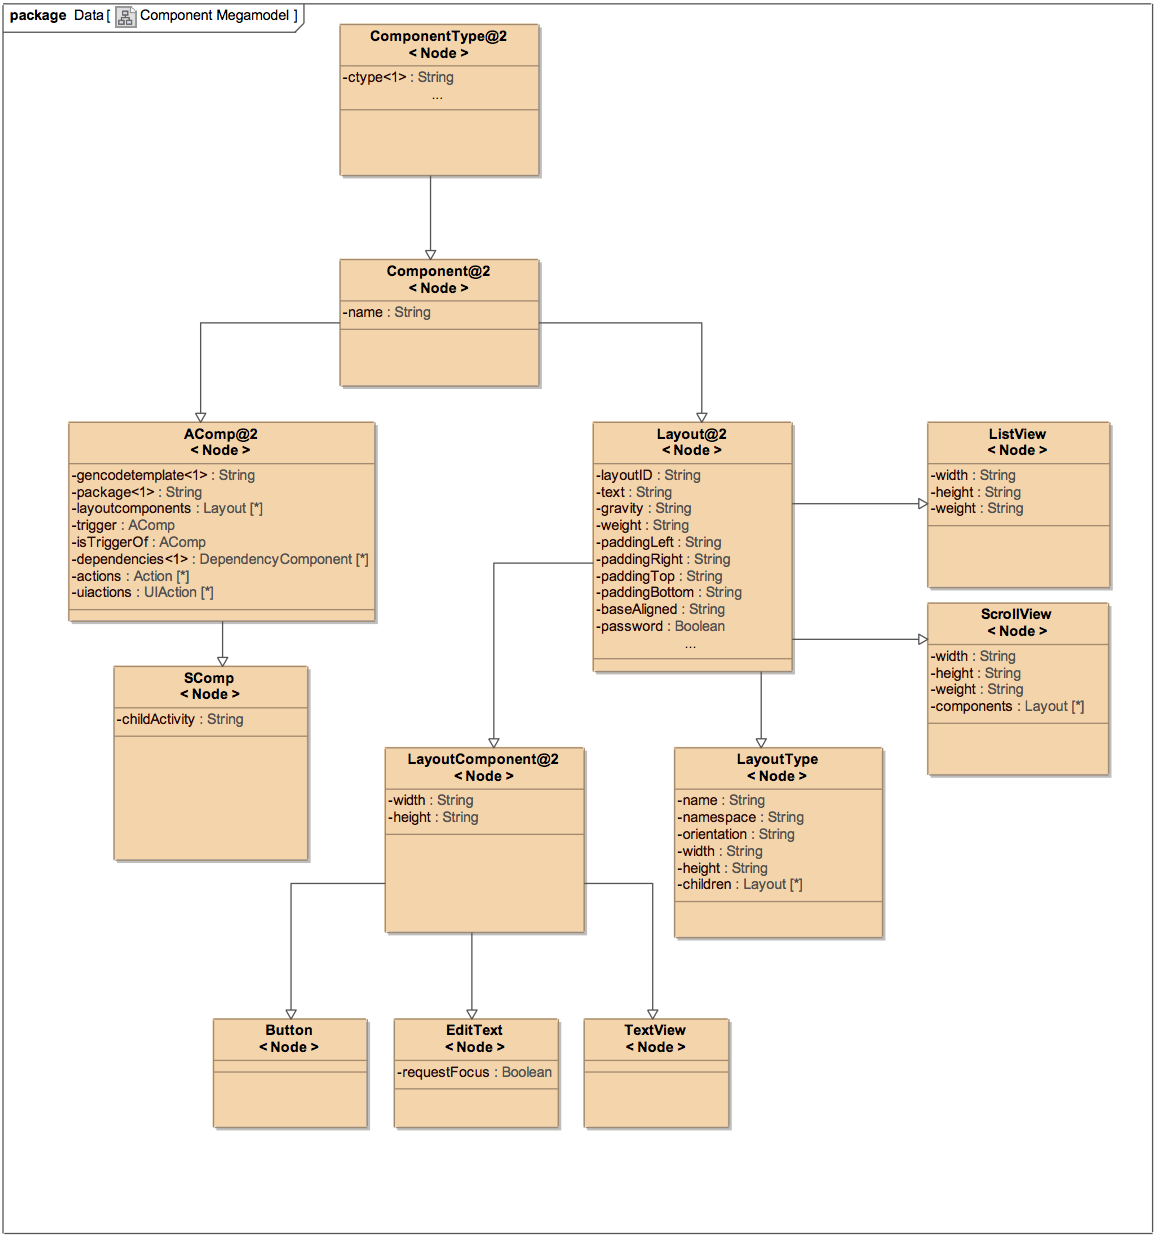
\includegraphics[width=1.0\textwidth]{images/chap6_component_megam.png}
\caption{Component Class Diagram}
\label{fig:component_megamodel}
\end{figure}

\subsection{Component}

The \texttt{Component} meta-model is listed in Listing ~\ref{component-mm}.

\begin{lstlisting}[label=component-mm,caption=Component meta-model, captionpos=t]
Model Component@2 {
	
	abstract Node ComponentType {
		ctype@1		: String{id};
	}

	Node Component : ComponentType {
		name			: String;
	}

	Node ComponentData@1 {
		name 		: String;
		value 		: String;
	}
	
	Node Layout : Component {
		layoutID		: String;
		text 			: String;
		gravity			: String;

		paddingLeft 	: String;
		paddingRight	: String;
		paddingTop 		: String;
		paddingBottom 	: String;
		baselineAligned : String;
	}

	// e.g. Button, EditText, TextView, ...
	Node LayoutComponent@2 : Layout {
		width			: String;
		height			: String;
		weight			: String;
	}

}
\end{lstlisting}
As we can see, this meta-model has a potency level of 2. This means that we have three levels in the meta-model. At the highest level, we define an abstract \texttt{Component} meta-model. Going down one level, we have defined the \texttt{AndroidComponent} itself (e.g. \textit{SMS}) and at level 0, we instantiate the component in our model. All components are of type \texttt{AndroidComponent} which is a subtype of \texttt{Component}. This component will be discussed in the next section. \texttt{LayoutComponent} is another component that inherits from our \texttt{Component} meta-model. It is used to describe the layout elements of an \texttt{Activity} and has a potency of two. It follows the same instantiation scheme as an \texttt{AndroidComponent} does.

\subsection{AndroidComponent}

\begin{lstlisting}[label=androidcomponent-mm,caption=AndroidComponent meta-model, captionpos=t]
load "Component"
load "AndroidAction"
load "UIAction"

Model AndroidComponent@2 imports Component, AndroidAction, UIAction {

	// Android component for semantics and extensibility
	Node AComp : Component {
		gencodetemplate@1 		: String;

		package@1 				: String;
		layoutcomponents@2 		: LayoutComponent@0[*];

		// Trigger can be another component (e.g. GeoComponent)
		trigger 				: AComp@0;

		// isTriggerOf defines the bi-directional connection with another component
		// a component could be the trigger of another component or a layoutcomponent
		isTriggerOf 			: AComp@0;
		dependencies@1 			: DependencyComponent[*];

		properties@1 			: ComponentData[*];
		
		// actions extend the action() method, so users can extend a component's functionality
		actions 				: Action[*];
		// uiactions are actions on a layoutcomponent
		uiactions 				: UIAction[*];
	}

	Edge Trigger@(2)(AComp.trigger, AComp.isTriggerOf) {
		actions 				: Action[*];
	}

	Node SComp : AComp {
		childActivity	: String;
	}
}
\end{lstlisting}
The \texttt{AndroidComponent} meta-model contains a \texttt{Node} that inherits from \texttt{Component}. \texttt{AComp} contains all necessary slots to instantiate and generate an Android component. At potency level one, we instantiate the EGL template to be used for generating the component code (in Java), the Java package that should be used, optional dependencies (regular Java classes) or properties to be associated with the component. An example of a possible property is a telephone number for sending an SMS. At the instantiation level, we can instantiate the remaining fields of \texttt{AComp}, such as \textit{layoutcomponents} or \textit{actions}. A \texttt{trigger} or \texttt{isTriggerOf} field can be specified, which enables local communication between two components. For example, when the trigger of a \texttt{GeoComponent} is fired, it passes its location to another component (e.g. \texttt{SMSComponent}), after which this component can use the location data to perform an action (e.g. send an SMS). This trigger can additionally be extended by using the \texttt{Trigger} edge. Through the \texttt{Trigger} edge, we can specify a list of actions to be executed when a trigger is fired. The trigger behavior is implicit to each component and cannot be changed. For instance, a \texttt{GeoComponent} will only trigger when a new location is found. \\ \\
Apart from a normal \texttt{AComp} node, a modeler can also instantiate components of type \texttt{SComp}. These components are used to represent client/server components. Typically, an instantiation of \texttt{SComp} communicates with a server. An example of this is the \texttt{DropboxComponent}. These type of components are usually embedded in an activity and could optionally have a child activity. For instance in a \texttt{DropboxComponent}, we usually want to show additional information on documents found in a Dropbox repository. This additional information will be shown through a child activity that is specified in a Dropbox instantiation of type \texttt{SComp}. \\

\subsection{Example Component}

As an example, we will show the Dropbox component, both on potency level one as well as on the instantiation level. The model for potency level one is listed in Listing ~\ref{dropbox-m}.

\begin{lstlisting}[label=dropbox-m,caption=Dropbox model, captionpos=t]
load "Component"

AndroidComponent dropboxComponent {
	
	SComp Dropbox {
		ctype = "dropbox";
		gencodetemplate = "dropbox.egl";

		folder 		: String;
		key 		: String;
		secret 		: String;
	}

}
\end{lstlisting}
At this level, we specify the template to generate the Java Dropbox component. We also introduce new slots that represent the name of the folder that should be used as a repository, together with the token key and token secret to authenticate with OAuth \cite{OAuth}. This level should and will never be visible to a developer. A modeler is only concerned about the instantiation level. The model instantiation is listed in Listing ~\ref{dropbox-inst}.

\begin{lstlisting}[label=dropbox-inst,caption=Dropbox instantiation, captionpos=t]
Dropbox dropbox {
	layoutcomponents = [dropboxButton, dirContentButton, contentText, dirContent];
	actions = [];
	uiactions = [triggerDropbox];

	childActivity = "DropboxItemActivity";
	folder = "/Thesis/";
	key = "KEY";
	secret = "SECRET";
}
\end{lstlisting}
We have defined a few layout components that make up the layout of the Dropbox activity. For instance, the \texttt{dirContentButton} value is used to grab the content of the Dropbox folder and the \texttt{dirContent} value represents the list that contains all filenames after the content is fetched from the Dropbox folder, that is specified by the folder, key and secret fields. When clicking on an item in a list, the activity that is specified in the \texttt{childActivity} field is initiated. This activity allows a user to make comments on a file (e.g. a research paper) in the specified Dropbox folder.

\section{Server}

In this section, we will review the \texttt{Server} meta-model and very briefly discuss the implementation details. The server component was written in Javascript and uses WebSockets for bi-directional communication, i.e. communication from client to server and vice versa.

\subsection{Meta-model}

The \texttt{Server} meta-model is quite straight-forward and the more complex parts are implemented in Node.js. \texttt{Server} is embedded into the \texttt{Application} meta-model. The code is listed in Listing ~\ref{server-mm}.

\begin{lstlisting}[label=server-mm,caption=Server meta-model, captionpos=t]
load "Session"
load "AndroidComponent"

Model Server imports Session, AndroidComponent {

	Node Server {
		name 			: String;
		session 		: SessionObject;
		host 			: String;
		port 			: String;
		components 		: Component@0[*];
	}
}
\end{lstlisting}
The host and port for the server can be set, together with the components that should be included in the server. Apart from that, a modeler should also set a \texttt{SessionObject} node. This node simply contains a list of users that are able to authenticate to the server, together with their role. 

\subsection{Javascript and WebSockets}

The most relevant part of the \texttt{Server} meta-model lies in the implementation in Javascript. In order to realize both asynchronous as well as synchronous communication, Node.js \cite{NodeJS} was used together with WebSockets:
\begin{quotation}
The WebSocket specification - developed as part of the HTML5 initiative - introduced the WebSocket JavaScript interface, which defines a full-duplex single socket connection over which messages can be sent between client and server. The WebSocket standard simplifies much of the complexity around bi-directional web communication and connection management \cite{WebSockets}. 
\end{quotation}
If we send all our data packets through a \texttt{WebSocket}, we can communicate with our server in \textit{near real-time}, because there is bi-directional communication between the client and server. Combining this with a server implementation in Node.js, we leverage Javascript to implement a data-intensive real-time application suited for multiple devices:
\begin{quotation}
Node.js is a platform built on Chrome's JavaScript runtime for easily building fast, scalable network applications. Node.js uses an event-driven, non-blocking I/O model that makes it lightweight and efficient, perfect for data-intensive real-time applications that run across distributed devices.
\end{quotation}
Since all communication works through WebSockets, the server implementation is decoupled from any Android application a developer may model. If at some point the modeling framework has to be adapted to generate iOS applications, nothing has to be changed to the Javascript server implementation. The only requirement is a \texttt{WebSocket} library on the client side (iOS/Android/web).

\section{Code Generation}

In this section, we will explain the code generation details of Metadepth and the collaborative modeling framework. First, we will briefly explain the Epsilon Generation Language (EGL) syntax. Afterwards, we will show an example of the code generation of the activities in an Android application.

\subsection{Epsilon Generation Language}

EGL is a template-based model-to-text language for generating code, documentation and other textual artefacts from models. EGL supports content-destination decoupling, protected regions for mixing generated with hand-written code, and template coordination \cite{EpsilonGenerationLanguage}. \\ \\
The concrete syntax of EGL closely resembles the style of other template-based code generation languages, such as PHP \cite{EpsilonBook}. Any text enclosed in a tag pair \textit{[\%} \textit{\%]} is used to delimit a dynamic code section. Text not inclosed in a tag pair is considered static code. Listing ~\ref{egl-template} illustrates the use of dynamic and static code sections to from a basic EGL template. 
\begin{lstlisting}[label=egl-template,caption=EGL template, captionpos=t]
?[% for (i in Sequence{1..5}) { %]
	i is [%= i %]
[% } %]
\end{lstlisting}
The structure of this basic template is used for the generation of Java code in the collaborative modeling framework. The next subsection shows an example of a real EGL template used in the collaborative modeling framework.

\subsection{Example}

Finally, after a model has been created, a developer can initiate the code generation phase. This phase loads a set of EGL files and traverses each model that has been created. A typical code generation process is implemented as follows:

\begin{lstlisting}[label=codegen-app,caption=Android code-generation, captionpos=t]
// generate main Android app
var t : Template := TemplateFactory.load(basePath+'genActivity.egl');
if (application.activities.isDefined() and application.activities.size() > 0) {
	for (activity in application.activities) {
		if (activity.main == true) {
			"populating server var".println();
			if (application.server.isDefined()) {
				t.populate('server', application.server);
			}
		}
		t.populate('activity', activity);
		t.populate('application', application);
		t.populate('path', path);
		t.populate('basePath',    basePath);
		t.populate('compPath',    compPath);
		t.populate('codePath',	  codePath);
		t.process();
		t.generate(codePath + 'src/' + path + activity.name + '.java');
	
		var l : Template := TemplateFactory.load(basePath+'genDependency.egl');
		if (activity.content.isDefined() and activity.content.size() > 0) {
			for (c in activity.content) {
				if (c.dependencies.isDefined() and c.dependencies.size() > 0) {
					for (d in c.dependencies) {
						l.populate('dependency', d);
						l.populate('basePath',    basePath);
						l.populate('compPath',    compPath);
						l.process();
						l.generate(codePath + 'src/' + path + d.name + '.java');
					}
				}
			}
		}
	}
}
\end{lstlisting}
This listing iterates all defined activities and generates the Java \texttt{Activity} files. Lines 11 through 16 populate the template with variables we need to generate the target (Java) code. The \texttt{populate} method passes variables in the source formalism and map these onto a name. For example, in line 11, we assigned the activity variable to 'activity' in the EGL template that will be called. Line 17 processes all this information and line 18 finally calls the template we initiated in line 2. The template is initiated by calling the \texttt{generate} method. This method expects one parameter, the location on the file system of the file that is to be generated. As an example, listing ~\ref{codegen-list} lists the EGL template to generate the List component.
\begin{lstlisting}[label=codegen-list,caption=Android List Component code-generation, captionpos=t]
[% out.setContentType('Java'); %]
package [%= package %];

[% if (component.childActivity.isDefined()) { %]
	[%
		// generate new childActivity class
		var t : Template := TemplateFactory.load(compPath+'listChild.egl');
		t.populate('name', component.childActivity);
		t.populate('package', package);
		t.populate('basePath', basePath);
		t.populate('compPath', compPath);
		t.populate('codePath', codePath);
		t.process();
		t.generate(codePath+'src/' + path + component.childActivity + '.java');
	%]

	[%
		for (p in Presentation.all) {
			if (component.childActivity == p.activityname) {
				t := TemplateFactory.load(basePath+'genLayout.egl');
				t.populate('layout', p.layout);
				t.populate('basePath',    basePath);
				t.populate('compPath',    compPath);
				t.process();
				t.generate(codePath+'res/layout/' + p.layout.name + '.xml');
			}
		}
	%]
[% } %]

import java.util.ArrayList;
import java.util.HashMap;

import android.app.Activity;
import android.content.Intent;
import android.util.Log;
import android.view.View;
import android.widget.AdapterView;
import android.widget.ArrayAdapter;
import android.widget.Button;
import android.widget.EditText;
import android.widget.ListView;
import be.pds.thesis.AndroidComponent;
import be.pds.thesis.GenericActivity;
import be.pds.thesis.ServerConnection;

public class ListComponent extends AndroidComponent {

	private final String TAG = getClass().getName();
	private HashMap<String, Object> properties;
	private ArrayList<String> content;
	private Button addNoteButton;
	private EditText noteInput;
	private ListView noteOutput;

	public ListComponent(Activity a) {
		super(a);

		properties = new HashMap<String, Object>();
		properties.put("type", ((GenericActivity)parent).getClassName());
		properties.put("parent", "null");
		content = new ArrayList<String>();
		
		addNoteButton = (Button) parent.findViewById(R.id.addNoteItemButton);
		noteInput = (EditText) parent.findViewById(R.id.noteItemInput);
		noteOutput = (ListView) parent.findViewById(R.id.noteContent);
		noteOutput.setOnItemClickListener(new AdapterView.OnItemClickListener() {

			@Override
			public void onItemClick(AdapterView<?> a, View v, int pos, long id) {
				String item = (String) noteOutput.getItemAtPosition(pos);
				String parent_mod = item.substring(0, item.length()-1);
				Log.i(TAG, "PARENT = " + parent_mod);
				Log.i(TAG, "Item " + parent_mod + " was clicked.");
				Intent i = new Intent(parent.getApplicationContext(), [%= component.childActivity %].class);
				i.putExtra("parent", parent_mod);
				i.putExtra("type", ((GenericActivity)parent).getClassName());
				
				parent.startActivityForResult(i, 0);
			}
			
		});
		
		ServerConnection.getInstance().getGenericNotes(properties);
		
		addNoteButton.setOnClickListener(new View.OnClickListener() {
			@Override
			public void onClick(View v) {
				properties.put("parent", "null");
				action(properties);
			}
		});
	}
	
	@Override
	public void action(HashMap<String, Object> properties) {
		properties.put("text", noteInput.getText().toString());
		ServerConnection.getInstance().addGenericNote(properties);
	}

	public void onMessage(final String message) {
		parent.runOnUiThread(new Runnable() {
			public void run() {
				content.add(message);
				String[] values = (String[])content.toArray(new String[content.size()]);
				ArrayAdapter<String> adapter = new ArrayAdapter<String>(parent.getApplicationContext(),
						android.R.layout.simple_list_item_1, values);
				noteOutput.setAdapter(adapter);
			}
		});
	}
}
\end{lstlisting}
The above code listing generates the child Activity for the List component. This child activity is an Activity that gets launched when a user clicks on an item in the List component. Next, it also generates the code. The remainder of the code listing contains the relevant code for the component itself. The component has a button to add notes (i.e. list items) and overrides the \texttt{onMessage} method from the \texttt{AndroidComponent} class. The button adds the new note to the layout and sends the content of the note to the server class for broadcasting to other users. The \texttt{onMessage} method gets called by the server class and adds new messages as list items to the layout. All implemented components inherit from the \texttt{AndroidComponent} class, which is defined as follows:
\begin{lstlisting}[label=androidcomponent-class,caption=AndroidComponent class, captionpos=t]
package be.pds.thesis;

import android.app.Activity;

import java.util.List;
import java.util.ArrayList;
import java.util.HashMap;

public abstract class AndroidComponent {
	
	protected List<AndroidAction> actions;
	protected Activity parent;
	private HashMap<String, Object> result;

	public AndroidComponent() {
		actions = new ArrayList<AndroidAction>();
	}

	public AndroidComponent(Activity parent) {
		actions = new ArrayList<AndroidAction>();
		this.parent = parent;
	}

	public void addAction(AndroidAction a) {
		actions.add(a);
	}

	public Activity getParent() {
		return this.parent;
	}

	abstract public void action(HashMap<String, Object> properties);
	
	abstract public void onMessage(final String message);
}
\end{lstlisting}
The abstract methods \texttt{action} and \texttt{onMessage} are implemented in every component that inherits from this one. The \texttt{actions} list is mainly used to execute additional actions on a component (such as manipulating UI elements). We also pass the parent Activity to the component, so that we can execute Android UI actions (such as showing a message when a user successfully sent a message or note to the server). The remainder of the source is included in the Github repository \footnote{https://github.com/philipdesmedt/Thesis-Android}.

\chapter{Case Study: Collaborative Knowledge-Management Platform}

In this chapter, we will discuss an example application of the collaborative modeling framework in detail. Using the framework, we built a model of a collaborative knowledge-management platform. This application allows several people to join a session and work together on a research project. Most of the components and collaborative patterns that are incorporated into the framework have been used in order to model this application. 

\section{Collaborative Knowledge-Management Platform}

The goal of this case study is the modeling of an application that shows the abilities of the collaborative modeling framework, but I also wanted to solve a real-life problem with it. The modeled application proposes a prototype that should make it easier for researchers to collaborate on research projects.

\subsection{Problem}

Currently, it is hard to work on a research project with multiple people. When reading papers, it is hard to make notes on them and it is not straightforward how to share those notes with other people. Currently, people make notes in the margin of a paper and pass this paper on to other people. This method does not encourage collaboration and it's hard to collaborate in real-time when both people want to read the same paper. This situation is one problem I wanted to fix with the collaborative platform. \\ \\
A second problem goes back to the collaboration in real-time. When two researchers are not in the same place (and/or time), it makes it hard to collaborate in real-time on a research project. How do people on one research project keep in sync all the time? We currently have the technology, we only need to build the right tools with this technology. If we use this technology as an enabler to work more efficiently (i.e. create the tools), how will this make us more efficient on a research project?

\subsection{Solution}

It looks like that the problem as I analyzed it is twofold:
\begin{itemize}
\item{In order to solve the first problem, we can introduce an annotation layer on top of a repository. In the collaborative modeling framework, a repository is modeled using a Dropbox folder. The metadata of every item in this folder can be fetched and annotated with a note by one of the registered researchers of the application. This allows people to simultaneously share their insights on new papers.} 
\item{When we want to allow a group of researchers to truly collaborate in real-time when they are not in the same place, we have to introduce a way to make it possible to easily communicate with current technology constraints. This problem is solved by integrating a chat box that allows a team to have a discussion in real-time, whether they are in the same place at the same time or not.}
\end{itemize}
In addition to solutions to those problems, the case study also includes other mechanisms that create awareness between researchers and helps them identify their research goals. In the following section, implementation details of these needs and features will be discussed.

\section{Platform implementation}

The main entities of the model for the Collaborative Knowledge-Management Platform are the Android activities. These activities represent the main features found in the application. Each of those are embedded in the main \texttt{Application} object. We will discuss the most important activities in depth in this section. All source code can be found on Github\footnote{https://github.com/philipdesmedt/Thesis-Android} \cite{Github}.

\begin{itemize}
\item{LoginActivity}
\item{MainActivity}
\item{ListActivity}
\end{itemize} 

\subsection{LoginActivity}

The model for \texttt{LoginActivity} is listed as follows:

\begin{lstlisting}[label=login-model,caption=LoginActivity model, captionpos=t]
Activity act1 {
	name = "LoginActivity";
	main = true;

	content = [login];
	presentation = pres1;
}
\end{lstlisting}
Following the \texttt{Activity} meta-model, we have set the \texttt{LoginActivity} model to be the main \texttt{Activity} (which means it will be the first one to be started by the Android OS). As a component, we include a login component and set the layout (which contains two textfields to authenticate, one for the username and for the password, and a button to initiate the login action). The login component is defined as follows:

\begin{lstlisting}[label=logincomponent-model,caption=Login component model, captionpos=t]
Login login {
	host = "10.0.2.2";
	port = "3000";

	layoutcomponents = [usernameView, usernameText, passwordView, passwordText, loginButton];
	actions = [ela1, ela2];
	uiactions = [triggerLogin];
}
\end{lstlisting}
Both the \texttt{host} and \texttt{port} fields are settings that should be set to connect to the server. The layout components are, as mentioned earlier, the inputs for authentication with the server. The \texttt{actions} list  extends the functionality of the \texttt{action} method of a component and the \texttt{uiactions} list contains actions that will be executed on UI elements. In the login component, \texttt{ela1} and \texttt{ela2} are both \texttt{ExtractLayoutAction} elements that extract both the username and the password from UI elements and use these in the \texttt{action} method to pass our credentials to the server. The UI action \texttt{triggerLogin} specifies what has to be done when the login button is triggered. This specific action effectively calls the \texttt{action} method of our login component and changes the Activity to \texttt{MainActivity} when the given credentials are verified. If the credentials are incorrect, nothing happens at all.

\subsection{MainActivity}

The \texttt{MainActivity} class is the entry point for our application once the user is logged in successfully. It contains shortcuts to all functionality within the app. This activity is modeled as follows:

\begin{lstlisting}[label=main-model,caption=MainActivity model, captionpos=t]
MainActivity act2 {
	name = "MainActivity";
	main = false;

	content = [twitter];
	presentation = pres2;
	onClickListeners = [triggerChat, triggerDropbox, triggerGoals, triggerLogout];
	userView = connectedUsers;
}
\end{lstlisting}
We only modeled one component in \texttt{MainActivity}, a Twitter component. We don't want a separate Activity for a Twitter component, so that's why we just embedded it into the current Activity and used a \texttt{Button} as a trigger for it. Because this component is offered as a complete integration, this \texttt{Button} is not included in the onClickListeners, but in the Twitter component itself. Because this component does not need a lot of customizations (apart from the text to tweet), it is offered as an integrated component solution in the framework. The onClickListeners specify all shortcuts to the other Activities in the current Activity. Finally, we also specified a \texttt{userView} field that, if set, shows all currently connected users in the application. \\ \\
Note that we don't just use the \texttt{Activity} meta-model, but the \texttt{MainActivity} meta-model. This meta-model has no difference with the \texttt{Activity} meta-model on a modeling level, but it has some differences on the implementation level. The \texttt{MainActivity.java} implementation inherits from the \texttt{Activity} implementation included in the Android SDK. Moreover, it is an \texttt{abstract class} that asks for the implementation of the \texttt{setConnectedUsers} method. This method takes a \texttt{String} of users as input and allows a modeler to show the currently connected users. That way, our collaborative framework can easily support the awareness of users in a collaborative application.

\subsection{ListActivity}

Another important Activity is the model of the \texttt{ListActivity}. We use this generic Activity to allow the implementation of lists of various forms in our application. This way we could model the annotation of Dropbox notes, a list of goals or a questionnaire that can have an arbitrary number of answers. The model for this generic activity is listed in listing ~\ref{list-model}.
\begin{lstlisting}[label=list-model,caption=ListActivity model, captionpos=t]
GenericActivity act5 {
	name = "ListActivity";
	main = false;

	content = [list];
	presentation = pres5;
}
\end{lstlisting}
The most important aspect of this model is the use of the \texttt{GenericActivity} type. Just like the \texttt{MainActivity}, this meta-model has no difference with the \texttt{Activity} meta-model, but the implementation again is slightly different. \texttt{GenericActivity} is an abstract class that has two abstract methods, \texttt{AndroidComponent getComponent()} and \texttt{void onMessage(String user, String message)}. The \texttt{getComponent()} method is used when we need to notify the embedded component within this Activity and the \texttt{onMessage()} method is a callback function that is called when we receive a message from the server. Usually, those \texttt{GenericActivity} classes also have a child Activity associated with them. This is true for our list component too. This child activity is used to display the comments or notes on a particular list item. For instance, if we model a list of goals, we can comment on these goals. These comments are wrapped into the child activity.

\section{Demonstration}

In this section, we will have a look at the running modeled application. In the previous section, the several activities and their models were discussed and now we can see them in action. In figure ~\ref{fig:coll_connected}, we see the main activity after a user successfully logged in. In this activity, a user can navigate to all other activities in the collaborative application.
\begin{figure}[h!]
\centering
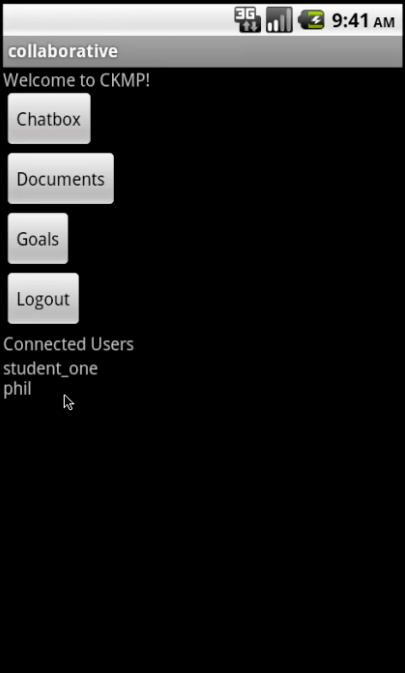
\includegraphics[width=0.4\textwidth]{images/chap7_connected.png}
\caption{In the main menu of the collaborative application with two connected users}
\label{fig:coll_connected}
\end{figure} \\
When we start the chat activity, a simple screen with the latest chat messages comes up. A user can send a message to all other users. This message will be persisted in the MongoDB database and subsequently sent to all users. A view of the chat box is depicted in figure ~\ref{fig:coll_chatbox}. 
\begin{figure}[h!]
\centering
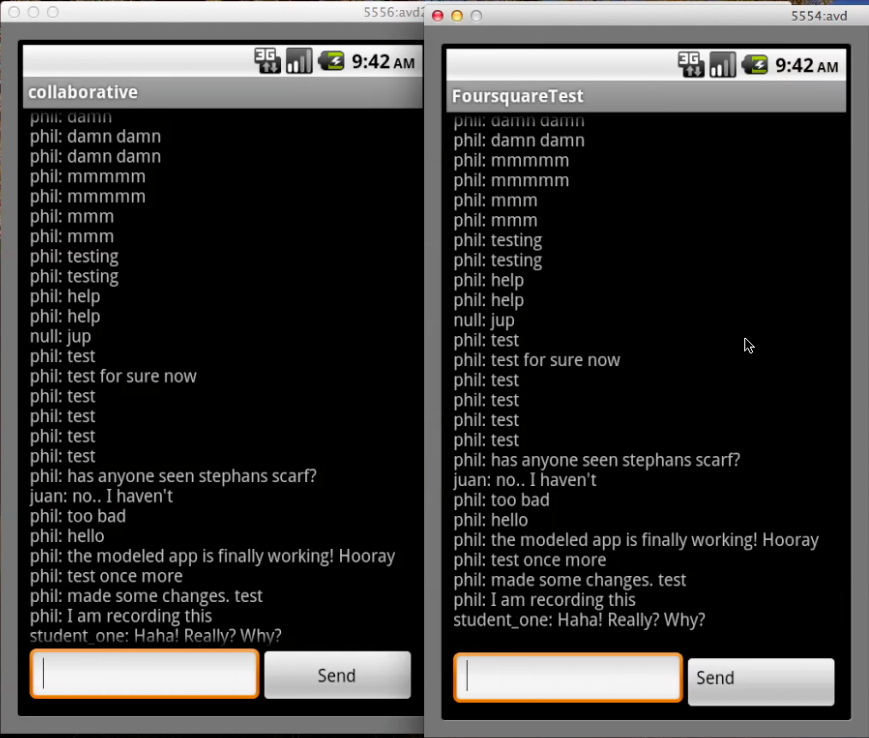
\includegraphics[width=0.99\textwidth]{images/chap7_chatbox.png}
\caption{In the chat box of the collaborative application}
\label{fig:coll_chatbox}
\end{figure} \\ 
Dropbox repository!
\begin{figure}[h!]
\centering
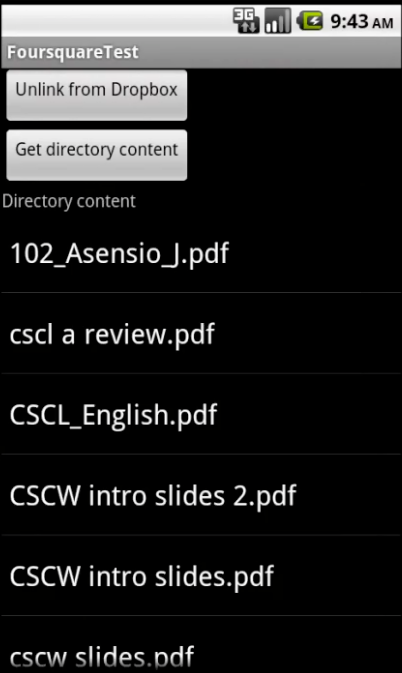
\includegraphics[width=0.4\textwidth]{images/chap7_dropbox1.png}
\caption{Fetched all research papers from the Dropbox repository}
\label{fig:coll_dropbox1}
\end{figure}
Notes on research paper in Dropbox repository!
\begin{figure}[h!]
\centering
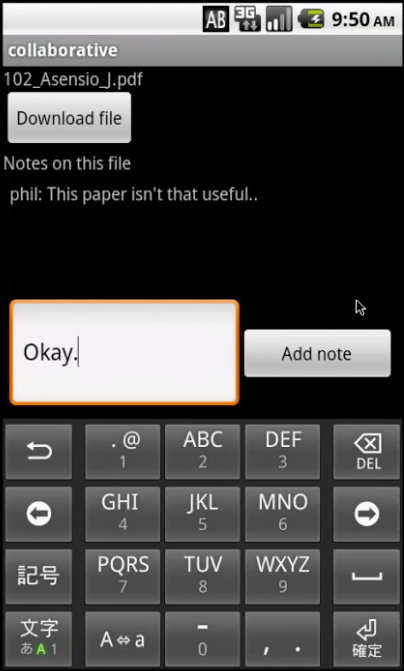
\includegraphics[width=0.4\textwidth]{images/chap7_dropbox2.png}
\caption{Notes and comments on a research paper in the Dropbox repository}
\label{fig:coll_dropbox2}
\end{figure}

\chapter{Conclusion}

\section{Summary}

\section{Future Work}


\begin{appendices}
\chapter{Meta-modeling and Petri Nets}
 
This chapter is an overview of the project done in the Petri Nets course.

\begin{table}[h]
\centering \begin{tabular}[]{l|l}
Bron & Resource \\
Bronbeheer-systemen & Resource Management Systems \\
...
\end{tabular}
\caption{Meta-modeling and Petri Nets}
\end{table}
\chapter{Model to model transformation [Research Internship 2]}
 
This chapter is an overview of the project done in the Petri Nets course.

\begin{table}[h]
\centering \begin{tabular}[]{l|l}
Bron & Resource \\
Bronbeheer-systemen & Resource Management Systems \\
...
\end{tabular}
\caption{Meta-modeling and Petri Nets}
\end{table}
\chapter{Commercial collaborative applications}
 
Commercial collaborative applications

\end{appendices}

\backpages
\end{document}
